%+++++++++++++++++++++++++++++++++++++++++++++++++++++++++++++++++++++++++++++++
%+++++++++++++++++++++++++++++++++++++++++++++++++++++++++++++++++++++++++++++++
%+++++++++++++++++++++++++++++++++++++++++++++++++++++++++++++++++++++++++++++++

%\mysubsection{Theory}

This section includes some material on notation, formulations and general theoretical backgrounds for \codeName .
Note that the formulation of nodes, objects, markers, etc. is presented right at the subsection of each object, see \refSection{sec:item:reference:manual}.
Furthermore, overview on the system assembly and system equations of motion is given in \refSection{sec:notationSystemOfEOM},
solvers are described in \refSection{sec:solvers}.

%+++++++++++++++++++++++++++++++++++++++++++++++++++++++++++++++++++++++++++++++++++++++++++
%+++++++++++++++++++++++++++++++++++++++++++++++++++++++++++++++++++++++++++++++++++++++++++
\mysubsection{Notation}
\label{sec:itemnotation}
%
\mysubsubsection{Common types in item descriptions}
\label{sec:typesDescriptions}
%
There are certain types, which are heavily used in the description of items:
\bi
  \item \texttt{float} $\ldots$ a single-precision floating point number (note: in Python, '\texttt{float}' is used also for double precision numbers; in EXUDYN, internally floats are single precision numbers especially for graphics objects and OpenGL)
  \item \texttt{Real} $\ldots$ a double-precision floating point number (note: in Python this is also of type '\texttt{float}')
  \item \texttt{UReal} $\ldots$ same as \texttt{Real}, but may not be negative
  \item \texttt{PReal} $\ldots$ same as \texttt{Real}, but must be positive, non-zero (e.g., step size may never be zero)
  \item \texttt{Index} $\ldots$ deprecated, represents unsined integer, \texttt{UInt}
  \item \texttt{Int} $\ldots$ a (signed) integer number, which converts to '\texttt{int}' in Python, '\texttt{int}' in C++
  \item \texttt{UInt} $\ldots$ an unsigned integer number, which converts to '\texttt{int}' in Python
  \item \texttt{PInt} $\ldots$ an positive integer number (> 0), which converts to '\texttt{int}' in Python
  \item \texttt{NodeIndex, MarkerIndex, ...} $\ldots$ a special (non-negative) integer type to represent indices of nodes, markers, ...; specifically, an unintentional conversion from one index type to the other is not possible (e.g., to convert \texttt{NodeIndex} to \texttt{MarkerIndex}); see \refSection{sec:itemIndex}
  \item \texttt{String} $\ldots$ a string
  \item \texttt{ArrayIndex} $\ldots$ a list of integer numbers (either list or in some cases \texttt{numpy} arrays may be allowed)
  \item \texttt{ArrayNodeIndex} $\ldots$ a list of node indices
  \item \texttt{Bool} $\ldots$ a boolean parameter: either \texttt{True} or \texttt{False} ('\texttt{bool}' in Python)
  \item \texttt{VObjectMassPoint}, \texttt{VObjectRigidBody}, \texttt{VObjectGround}, etc.  $\ldots$ represents the visualization object of the underlying object; 'V' is put in front of object name
  \item \texttt{BodyGraphicsData} $\ldots$ see \refSection{sec:graphicsData}
%	
	\item \texttt{Vector2D} $\ldots$ a list or \texttt{numpy} array of 2 real numbers
	\item \texttt{Vector3D} $\ldots$ a list or \texttt{numpy} array of 3 real numbers
	\item \texttt{Vector'X'D} $\ldots$ a list or \texttt{numpy} array of 'X' real numbers
	\item \texttt{Float4} $\ldots$ a list of 4 float numbers
%
	\item \texttt{Vector} $\ldots$ a list or \texttt{numpy} array of real numbers (length given by according object)
	\item \texttt{NumpyVector} $\ldots$ a 1D \texttt{numpy} array with real numbers (size given by according object); similar as Vector, but not accepting list

	\item \texttt{Matrix3D} $\ldots$ a list of lists or \texttt{numpy} array with $3 \times 3$ real numbers
	\item \texttt{Matrix6D} $\ldots$ a list of lists or \texttt{numpy} array with $6 \times 6$ real numbers
	\item \texttt{NumpyMatrix} $\ldots$ a 2D \texttt{numpy} array (matrix) with real numbers (size given by according object)
	\item \texttt{NumpyMatrixI} $\ldots$ a 2D \texttt{numpy} array (matrix) with integer numbers (size given by according object)
	\item \texttt{MatrixContainer} $\ldots$ a versatile representation for dense and sparse matrices, see \refSection{sec:MatrixContainer} below
  \item \texttt{PyFunctionGraphicsData} $\ldots$ a user function providing GraphicsData, see the user function description of the according object
  \item \texttt{PyFunctionMbsScalar...} $\ldots$ a user function for the according object; the name is chosen according to the interface (arguments containing scalars, vectors, etc.); see the according user function description
  %
\ei

\mysubsubsection{MatrixContainer} 
\label{sec:MatrixContainer}
The \texttt{MatrixContainer} is a versatile representation for dense and sparse matrices.
Some functionality:
\bi
  \item Create empty \texttt{MatrixContainer} with \texttt{mc = MatrixContainer()}
  \item Set with dense \text{pyArray} (a numpy array) (if \texttt{useDenseMatrix} is set False, it converts into a sparse matrix, which may speed up further computations for sparse matrices!): \texttt{mc.SetWithDenseMatrix(pyArray, bool useDenseMatrix = True)}
  \item Set with sparse \text{pyArray} (a numpy array), which has 3 colums and according rows containing the sparse triplets \texttt{(row, col, value)} describing the sparse matrix; Use \texttt{CSRtoScipySparseCSR(...)} and \texttt{ ScipySparseCSRtoCSR(...)} to convert between this format and the scipy csr format; if \texttt{useDenseMatrix} is set True, it converts into a dense matrix, which may slow down computations: \texttt{mc.SetWithSparseMatrixCSR(numberOfRowsInit, numberOfColumnsInit, pyArray, useDenseMatrix = False)}
  \item Convert matrix into dense format (slow, but helpful for debug): \texttt{mc.Convert2DenseMatrix()}
  \item Get internal stored object: \texttt{mc.GetPythonObject()}
  \item \mybold{Automatic type conversion}: if a function or class requests a \texttt{MatrixContainer}, such as \texttt{ObjectGenericODE2}, there are automatic type conversions from:
  \bi
    \item empty list: \texttt{[]}
    \item numpy array, e.g.: \texttt{np.array([[1,2],[3,4]])}
    \item list of lists describing matrix, e.g. (slow for larger matrices!): \texttt{[[1,2],[3,4]]}
  \ei
\ei

%
\mysubsubsection{States and coordinate attributes}
The following subscripts are used to define configurations of a quantity, e.g., for a vector of displacement coordinates $\qv$:
\bi
  \item $\qv\cConfig \ldots$ $\qv$ in any configuration
  \item $\qv\cRef \ldots$ $\qv$ in reference configuration, e.g., reference coordinates: $\cv\cRef$
  \item $\qv\cIni \ldots$ $\qv$ in initial configuration, e.g., initial displacements: $\uv\cIni$
  \item $\qv\cCur \ldots$ $\qv$ in current configuration
  \item $\qv\cVis \ldots$ $\qv$ in visualization configuration
  \item $\qv\cSOS \ldots$ $\qv$ in start of step configuration
\ei
As written in the introduction, the coordinates are attributed to certain types of equations and therefore, the following attributes are used (usually as subscript, e.g., $\qv_{ODE2}$):
\bi
  \item \hacs{ODE2} $\ldots$ \acl{ODE2} (coordinates)
  \item \hacs{ODE1} $\ldots$ \acl{ODE1} (coordinates)
  \item \hacs{AE} $\ldots$ \acl{AE} (coordinates)
  \item Data $\ldots$ data coordinates (history variables)
\ei
Time is usually defined as 'time' or $t$.
The cross product or vector product '$\times$' is often replaced by the skew symmetric matrix using the tilde '$\tilde{\;\;}$' symbol,
\be
  \av \times \bv = \tilde \av \, \bv = -\tilde \bv \, \av \eqComma
\ee
in which $\tilde{\;\;}$ transforms a vector $\av$ into a skew-symmetric matrix $\tilde \av$.
The inverse operation is denoted as $\vec$, resulting in $\vec(\tilde \av) = \av$.

For the length of a vector we often use the abbreviation 
\be \label{eq:definition:length}
  \Vert \av \Vert = \sqrt{\av^T \av} \eqDot
\ee

A vector $\av=[x,\, y,\, z]\tp$ can be transformed into a diagonal matrix, e.g.,
\be
  \Am = \diag(\av) = \mr{x}{0}{0} {0}{y}{0} {0}{0}{z} 
\ee
%
%+++++++++++++++++++++++++++++++++++++++++++++++++++++++++++++++++++++++++++++++++++++++++++
\mysubsubsection{Symbols in item equations}
\label{sec:symbolsItems}
\noindent The following table contains the common notation: \vspace{-12pt}
\begin{center}
  \footnotesize
  \begin{longtable}{| p{5cm} | p{5cm} | p{6cm} |}
    \hline
    \bf python name (or description) & \bf symbol & \bf description \\ \hline
    displacement coordinates (\hac{ODE2}) & $\qv = [q_0,\, \ldots,\, q_n]\tp$ & vector of $n$ displacement based coordinates in any configuration; used for second order differential equations\\ \hline
    rotation coordinates (\hac{ODE2}) & $\tpsi = [\psi_0,\, \ldots,\, \psi_\eta]\tp$ & vector of $\eta$ {\bf rotation based coordinates} in any configuration; these coordinates are added to reference rotation parameters to provide the current rotation parameters; used for second order differential equations\\ \hline
    coordinates (\hac{ODE1}) & $\yv = [y_0,\, \ldots,\, y_n]\tp$ & vector of $n$ coordinates for first order ordinary differential equations (\hac{ODE1}) in any configuration\\ \hline
    algebraic coordinates & $\zv = [z_0,\, \ldots,\, z_m]\tp$ & vector of $m$ algebraic coordinates if not Lagrange multipliers in any configuration\\ \hline
    Lagrange multipliers & $\tlambda = [\lambda_0,\, \ldots,\, \lambda_m]\tp$ & vector of $m$ Lagrange multipliers (=algebraic coordinates) in any configuration\\ \hline
    data coordinates & $\xv = [x_0,\, \ldots,\, x_l]\tp$ & vector of $l$ data coordinates in any configuration\\ \hline
%+++++++++++++++++++++++++++++++++++++++++++++++++++
    \hline %new part of table
		\bf python name: OutputVariable & \bf symbol & \bf description \\ \hline
    Coordinate & $\cv = [c_0,\, \ldots,\, c_n]\tp$ & coordinate vector with $n$ generalized coordinates $c_i$ in any configuration; the letter $c$ is used both for \hac{ODE1} and \hac{ODE2} coordinates\\ \hline
    Coordinate\_t & $\dot \cv = [c_0,\, \ldots,\, c_n]\tp$ & time derivative of coordinate vector\\ \hline
    Displacement & $\LU{0}{\uv} = [u_0,\, u_1,\, u_2]\tp$ & global displacement vector with 3 displacement coordinates $u_i$ in any configuration; in 1D or 2D objects, some of there coordinates may be zero\\ \hline
Rotation & $[\varphi_0,\,\varphi_1,\,\varphi_2]\tp\cConfig$ & vector with 3 components of the Euler angles in xyz-sequence ($\LU{0b}{\Rot}\cConfig=:\Rot_0(\varphi_0) \cdot \Rot_1(\varphi_1) \cdot \Rot_2(\varphi_2)$), recomputed from rotation matrix\\ \hline
    %Rotation & $\ttheta = [\theta_0,\, \ldots,\, \theta_n]\tp$ & vector of {\bf rotation parameters} (e.g., Euler parameters, Tait Bryan angles, ...) with $n$ coordinates $\theta_i$ in any configuration\\ \hline
    Identity matrix & $\Im = \mr{1}{0}{0} {0}{\ddots}{0} {0}{0}{1}$ & the identity matrix, very often $\Im = \ImThree$, the $3 \times 3$ identity matrix \\ \hline
    Identity transformation & $\LU{0b}{\ImThree} = \ImThree$ & converts body-fixed into global coordinates, e.g., $\LU{0}{\xv} = \LU{0b}{\ImThree} \LU{b}{\xv}$, thus resulting in $\LU{0}{\xv} = \LU{b}{\xv}$ in this case\\ \hline
    RotationMatrix & $\LU{0b}{\Rot} = \mr{A_{00}}{A_{01}}{A_{02}} {A_{10}}{A_{11}}{A_{12}} {A_{20}}{A_{21}}{A_{22}}$ & a 3D rotation matrix, which transforms local (e.g., body $b$) to global coordinates (0): $\LU{0}{\xv} = \LU{0b}{\Rot} \LU{b}{\xv}$\\ \hline
    RotationMatrixX & $\LU{01}{\Rot_0(\theta_0)} = 
		\mr{1}{0}{0} {0}{\cos(\theta_0)}{-\sin(\theta_0)} {0}{\sin(\theta_0)}{\cos(\theta_0)}$ & rotation matrix for rotation around $X$ axis (axis 0), transforming a vector from frame 1 to frame 0\\ \hline    
    %
		RotationMatrixY & $\LU{01}{\Rot_1(\theta_1)} = 
		\mr{\cos(\theta_0)}{0}{\sin(\theta_0)} {0}{1}{0} {-\sin(\theta_0)}{0}{\cos(\theta_0)}$ & rotation matrix for rotation around $X$ axis (axis 0), transforming a vector from frame 1 to frame 0\\ \hline    %
    RotationMatrixZ & $\LU{01}{\Rot_2(\theta_2)} = 
		\mr{\cos(\theta_0)}{-\sin(\theta_0)}{0} {\sin(\theta_0)}{\cos(\theta_0)}{0} {0}{0}{1}$ & rotation matrix for rotation around $X$ axis (axis 0), transforming a vector from frame 1 to frame 0\\ \hline    
		Position & $\LU{0}{\pv} = [p_0,\, p_1,\, p_2]\tp$ & global position vector with 3 position coordinates $p_i$ in any configuration\\ \hline
		Velocity & $\LU{0}{\vv} = \LU{0}{\dot \uv} = [v_0,\, v_1,\, v_2]\tp$ & global velocity vector with 3 displacement coordinates $v_i$ in any configuration\\ \hline
    AngularVelocity & $\LU{0}{\tomega} = [\omega_0,\, \ldots,\, \omega_2]\tp$ & global angular velocity vector with $3$ coordinates $\omega_i$ in any configuration\\ \hline
    Acceleration & $\LU{0}{\av} = \LU{0}{\ddot \uv} = [a_0,\, a_1,\, a_2]\tp$ & global acceleration vector with 3 displacement coordinates $a_i$ in any configuration\\ \hline
    AngularAcceleration & $\LU{0}{\talpha} = \LU{0}{\dot \tomega} = [\alpha_0,\, \ldots,\, \alpha_2]\tp$ & global angular acceleration vector with $3$ coordinates $\alpha_i$ in any configuration\\ \hline
%
    VelocityLocal & $\LU{b}{\vv} = [v_0,\, v_1,\, v_2]\tp$ & local (body-fixed) velocity vector with 3 displacement coordinates $v_i$ in any configuration\\ \hline
    AngularVelocityLocal & $\LU{b}{\tomega} = [\omega_0,\, \ldots,\, \omega_2]\tp$ & local (body-fixed) angular velocity vector with $3$ coordinates $\omega_i$ in any configuration\\ \hline
    Force & $\LU{0}{\fv} = [f_0,\, \ldots,\, f_2]\tp$ & vector of $3$ force components in global coordinates\\ \hline
    Torque & $\LU{0}{\ttau} = [\tau_0,\, \ldots,\, \tau_2]\tp$ & vector of $3$ torque components in global coordinates\\ \hline
%+++++++++++++++++++++++++++++++++++++++++++++++++++
		\hline %new part of table
    \bf python name: input to nodes, markers, etc. & \bf symbol & \bf description \\ \hline
    referenceCoordinates & $\cv\cRef = [c_0,\, \ldots,\, c_n]\cRef\tp = [c_{\mathrm{Ref},0},\, \ldots,\, c_{\mathrm{Ref},n}]\cRef\tp$ & $n$ coordinates of reference configuration (can usually be set at initialization of nodes)\\ \hline
    initialCoordinates & $\cv\cIni$ & initial coordinates with generalized or mixed displacement/rotation quantities (can usually be set at initialization of nodes)  \\ \hline
    reference point & $\pRefG = [r_0,\, r_1,\, r_2]\tp$ & reference point of body, e.g., for rigid bodies or \hac{FFRF} bodies, in any configuration; NOTE: for ANCF elements, $\pRefG$ is used for the position vector to the beam centerline\\ \hline    
    localPosition & $\pLocB = [\LUR{b}{b}{0},\, \LUR{b}{b}{1},\, \LUR{b}{b}{2}]\tp$ & local (body-fixed) position vector with 3 position coordinates $b_i$ in any configuration, measured relative to reference point; NOTE: for rigid bodies, $\LU{0}{\pv} = \pRefG + \LU{0b}{\Rot} \pLocB$;
		localPosition is used for definition of body-fixed local position of markers, sensors, COM, etc.\\ \hline
	  \end{longtable}
	\end{center}
%
%+++++++++++++++++++++++++++++++++++++++++++++++++++++++++++++++++++++++++++++++++++++++++++
%+++++++++++++++++++++++++++++++++++++++++++++++++++++++++++++++++++++++++++++++++++++++++++
\mysubsubsection{Reference and current coordinates}
%
An important fact on the coordinates is upon the splitting of quantities (e.g. position, rotation parameters, etc.) into reference and current (initial/visualization/...) coordinates.
The current position vector of a point node is computed from the reference position plus the current displacment, reading
\be
  \pv\cCur = \pv\cRef + \uv\cCur
\ee
In the same way rotation parameters are computed from,
\be
  \ttheta\cCur = \ttheta\cRef + \tpsi\cCur
\ee
which are based on reference quantities plus displacements or {\it changes}. Note that these changes are additive, even for rotation parameters. Needless to say, $\tpsi\cCur$ do not represent rotation parameters, while $\ttheta\cRef$ should be chosen such that they represent the orientation of a node in reference configuration.
The necessity for reference coordinates originates from finite elements, which usually split nodal position into displacements and reference position.
However, we also use the reference position here in order to define joints, e.g., using the utility function \texttt{AddRevoluteJoint(...)}.

Against to the splitting of positions, displacements and velocities (and most other quantities) are not having this reference part!

\mysubsubsection{Reference point}
%
In contrast to the reference position or reference coordinates, the reference point is mainly used for objects, e.g., rigid bodies.
The reference point is the position of the underlying (rigid body) node, while we can compute the position of any point on the body (or on the mass point).
The reference point is also the origin of the co-rotating (reference) frame with the body-fixed coordinate system.

The same concept is also used for \hac{FFRF} objects. In most cases, reference points are denoted by $\pRef$.

%+++++++++++++++++++++++++++++++++++++++++++++++++++++++++++++++++++++++++++++++++++++++++++
\mysubsubsection{Coordinate Systems}
%
\noindent The left indices provide information about the coordinate system, e.g.,
\be
  \LU{0}{\uv}
\ee
is the displacement vector in the global (inertial) coordinate systme $0$, while 
\be
  \LU{m1}{\uv}
\ee
represents the displacement vector in marker 1 ($m1$) coordinates. Typical coordinate systems:
\bi
  \item $\LU{0}{\uv}$ $\ldots$ global coordinates
  \item $\LU{b}{\uv}$ $\ldots$ body-fixed, local coordinates
  \item $\LU{m0}{\uv}$ $\ldots$ local coordinates of (the body or node of) marker $m0$
  \item $\LU{m1}{\uv}$ $\ldots$ local coordinates of (the body or node of) marker $m1$
  \item $\LU{J0}{\uv}$ $\ldots$ local coordinates of joint $0$, related to marker $m0$
  \item $\LU{J1}{\uv}$ $\ldots$ local coordinates of joint $1$, related to marker $m1$
\ei
To transform the local coordinates $\LU{m0}{\uv}$ of marker 0 into global coordinates $\LU{0}{\xv}$, we use
\be
  \LU{0}{\uv} = \LU{0,m0}{\Rot} \LU{m0}{\uv}
\ee
in which $\LU{0,m0}{\Rot}$ is the transformation matrix of (the body or node of) the underlying marker 0.

\mysubsubsection{Integration Points}
\label{sec:integrationPoints}
For several tasks, especially for finite elements and contact, different integration rules are used, which are summarized here.
The interval of all integration rules is $\in [-1,1]$, thus giving a total sum for integration weights of 2.
The points $\xi_{ip}$ and weights $w_{ip}$ for Gauss rules read:
\begin{center}
  \footnotesize
  \begin{longtable}{| c | c | c | c | c |}
    \hline
    type/order & point 0 & point 1 & point 2 & point 3 \\ \hline
    %Gauss 7 & \\ \hline
    Gauss 1 & 0 & & &\\ \hline
    Gauss 3 & $-\sqrt{1 / 3}$ & $\sqrt{1 / 3}$ & &\\ \hline
    Gauss 5 & $-\sqrt{3 / 5}$ & 0 & $\sqrt{3 / 5}$ &\\ \hline
    Gauss 7 & $-\sqrt{3 / 7 + \sqrt{120} / 35}$ & $-\sqrt{3 / 7 - \sqrt{120} / 35}$ & $\sqrt{3 / 7 - \sqrt{120} / 35}$ & $\sqrt{3 / 7 + \sqrt{120} / 35}$ \\ \hline
    \hline
    type/order & weight 0 & weight 1 & weight 2 & weight 3 \\ \hline
    Gauss 1 & 2 & & &\\ \hline
    Gauss 3 & 1 & 1 & &\\ \hline
    Gauss 5 & $5 / 9$ & $8 / 9$ & $5 / 9$ & \\ \hline
    Gauss 7 & $1 / 2 - 5 / (3 \sqrt{120})$ & $1 / 2 + 5 / (3*\sqrt{120})$ & $1 / 2 + 5 / (3*\sqrt{120})$ & $1 / 2 - 5 / (3*\sqrt{120})$ \\ \hline
  \end{longtable}
\end{center}
The points $\xi_{ip}$ and weights $w_{ip}$ for Lobatto rules read:
\begin{center}
  \footnotesize
  \begin{longtable}{| c | c | c | c | c |}
    \hline
    type/order & point 0 & point 1 & point 2 & point 3 \\ \hline
    Lobatto 2 & -1 & 1 & &\\ \hline
    Lobatto 4 & -1 & 0 & 1&\\ \hline
    Lobatto 6 & -1& $-\sqrt{1/5}$ & $\sqrt{1/5}$& 1\\ \hline
    \hline
    type/order & weight 0 & weight 1 & weight 2 & weight 3 \\ \hline
    Lobatto 2 & 1 & 1 & &\\ \hline
    Lobatto 4 & $1/3$& $4/3$& $1/3$&\\ \hline
    Lobatto 6 & $1/6$& $5/6$& $5/6$& $1/6$\\ \hline
  \end{longtable}
\end{center}
Further integration rules can be found in the C++ code of \codeName\ , see file \texttt{BasicLinalg.h}.



%+++++++++++++++++++++++++++++++++++++++++++++++++++++++++++++++++++++++++++++++++++++++++++
\newpage
\mysubsection{Model order reduction and component mode synthesis}
\label{sec:theory:CMS}
%terminology: eigenmode, eigenvector, eigenvalue, normal mode, static mode

This section describes the process how to create general flexible multibody system models using the floating frame of reference formulation with model order reduction (here also denoted as \hac{CMS}). The according object \texttt{ObjectFFRFreducedOrder} is described in \refSection{sec:item:ObjectFFRFreducedOrder}.

\mysubsubsection{Eigenmodes}
This section will describe the computation of eigenmodes using FEMinterface.

The \texttt{FEMinterface} in the module \texttt{FEM} has various functionality to import finite element meshes from finite element software.
We create a \texttt{FEMinterface} by means of
\bi
  \item[] \texttt{fem = FEMinterface()}
\ei
which allows us to use the variable \texttt{fem} from now.

Meshes can be imported from NETGEN/NGsolve (\refSection{sec:FEM:FEMinterface:ImportMeshFromNGsolve}), Abaqus (see \refSection{sec:FEM:FEMinterface:ImportFromAbaqusInputFile} and other sections related to ABAQUS), ANSYS (see \refSection{sec:FEM:FEMinterface:ReadElementsFromAnsys} and other sections related to ANSYS).
The import procedure, which can also be done manually, needs to include \texttt{massMatrix} $\Mm$ and \texttt{stiffnessMatrix} $\Km$ from any finite element model.
Note that many functions are based on the requirement that nodes are 3D displacement-based nodes, without rotation or other coordinates.

For any functionality with \texttt{ObjectFFRFreducedOrder} and for the computation of Hurty-Craig-Bampton modes as described in the next section, \texttt{nodes}
are required.
Finally, \texttt{elements} need to be included for visualization, and a surface needs to be reconstructed from the element connectivity, which is available for tetrahedral and hexahedral elements for most import functions.

%++++++++++++++++++++++++
\begin{figure}[tbph]
  \begin{center}
  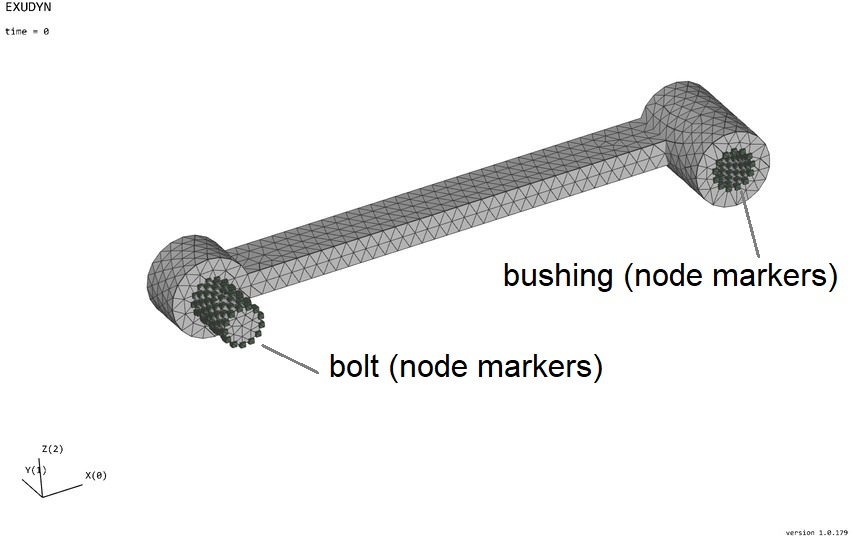
\includegraphics[width=10cm]{figures/modesHinge/HCBhingeMesh.jpg}
  \end{center}
  \caption{Test model and mesh for hinge created with Netgen (linear tetrahedral elements).}
	\label{fig_hingePartMesh}
\end{figure}
%++++++++++++++++++++++++
As an example, we consider a part denoted as 'hinge' in the following, see \fig{fig_hingePartMesh}. The test example can be found in \texttt{Examples/NGsolveCMStutorial.py} with lots of additional features.

After import of mass and stiffness matrix, eigenmodes and eigenfrequencies can be computed using \texttt{fem.ComputeEigenFrequencies(...)}, 
which computes the quantities \texttt{fem.modeBasis} and \texttt{fem.eigenValues}.
The eigenvalues in Hz can be retrieved also with the function \texttt{fem.GetEigenFrequenciesHz()}.
The function \texttt{fem.ComputeEigenFrequencies(...)} is available for dense and sparse matrices, and uses \texttt{scipy.linalg} to compute eigenvalues of the linear, undamped mechanical system
\be \label{theory:eigenmodes:EOM}
	\Mm \ddot \qv(t) + \Km \qv(t) = \fv(t) \eqDot
\ee
Here, the total number of coordinates of the system is $n$, 
thus having the vector of system coordinates $\qv \in \Rcal^n$, 
vector of applied forces $\fv \in \Rcal^n$, 
mass matrix $\Mm \in \Rcal^{n \times n}$ and stiffness matrix $\Km \in \Rcal^{n \times n}$. 
If we are interested in free vibrations of the system, without any boundary conditions or interconnections to other bodies, \eq{theory:eigenmodes:EOM} can be converted to a generalized eigenvalue problem. Using the approach 
$\qv(t) = \vv \mathrm{e}^{\mathrm{i} \omega t}$ in \eq{theory:eigenmodes:EOM}, and thus $\ddot \qv(t) = -\omega^2 \qv(t)$, we obtain
\be \label{theory:eigenmodes:harmonicEquation}
		\left[ \left(-\omega^2 \Mm + \Km \right) \vv \right] \mathrm{e}^{i\omega t} = \Null \eqDot
\ee
Assuming that \eq{theory:eigenmodes:harmonicEquation} is valid for all times, the {\bf generalized eigenvalue problem} follows that
\be \label{theory:eigenmodes:GEP}
	\left(-\omega^2 \Mm + \Km \right) \vv = \Null \eqComma
\ee
which can be rewritten as
\be \label{theory:eigenmodes:GEP2}
	\det \left(-\omega^2 \Mm + \Km \right) = 0 \eqComma
\ee
and which defines the eigenvalues $\omega_i^2$ of the linear system, where $i \in \{0, \ldots, n-1\}$. Note that in this case, the eigenvalues are the squared eigenfrequencies (in rad/s).
We can use eigenvalue algorithms to compute the eigenvalues $\omega_i^2$ and according eigenvectors $\vv_i$ from Python.
The function \texttt{fem.ComputeEigenmodes(...)} uses \texttt{eigh(...)} from \texttt{scipy.linalg} in the dense matrix mode, 
and in the sparse mode \texttt{eigsh(...)} from \texttt{scipy.sparse.linalg}, the latter being restricted to pure symmetric matrices.
Using special shift-inverted techniques in \texttt{eigsh(...)}, it performs much better than standard settings. However, you may tune your specific eigenvalue problem by modifying the solver procedure (just copy that function and adjust to your needs).
As an output, we obtain the smallest \texttt{nModes} eigenvectors (=eigenmodes)\footnote{Eigenvectors are the result of the eigenvalue algorithm, such as the QR algorithm. The mechanical interpretation of eigenvectors are eigenmodes, that can be visualized as shown in the figures of this section.} of the system.
Here, we will also use synonymously the terms `eigenmodes' and `normal modes', which result from an eigenvalue/eigenvector computation using certain (or even no) boundary conditions.
%++++++++++++++++++++++++
\begin{figure}[tbph]
  \begin{center}
  \includegraphics[width=4cm]{figures/modesHinge/freeFreeModeStress1}
  \includegraphics[width=4cm]{figures/modesHinge/freeFreeModeStress2}
  \includegraphics[width=4cm]{figures/modesHinge/freeFreeModeStress3}
  \includegraphics[width=4cm]{figures/modesHinge/freeFreeModeStress4}\\
  \includegraphics[width=4cm]{figures/modesHinge/freeFreeModeStress5}
  \includegraphics[width=4cm]{figures/modesHinge/freeFreeModeStress6}
  \includegraphics[width=4cm]{figures/modesHinge/freeFreeModeStress7}
  \includegraphics[width=4cm]{figures/modesHinge/freeFreeModeStress8}
  \end{center}
  \caption{Lowest 8 free-free modes for hinge finite element model, contour plot for $xx$-stress component.}
	\label{fig_hingePartFreeFreeModes}
\end{figure}
%++++++++++++++++++++++++

Clearly, if there are no supports included in the stiffness matrix, the resulting eigenmodes will contain 6 rigid body modes and we will also call this case for the computation of eigenmodes the `free-free' case, in analogy to a simply supported beam.
This rigid body modes, which are usually not needed (=unwanted) in the succeeding computation, can be excluded with an according option in \vspace{6pt}\\
\texttt{fem.ComputeEigenFrequencies(excludeRigidBodyModes = ...)}
\vspace{12pt}\\
For our test example, 8 eigenmodes are shown in \fig{fig_hingePartFreeFreeModes}, where the 6 rigid body modes have been excluded (so in total, 14 eigenvectors were computed).
%free free modes (coarse mesh, nNodes= 1216):
%freq(Hz)=[ 671.59137506  707.17488417 1298.50905491 1929.97563131 1971.76505866
%3141.47119938 3595.34508711 4317.51987533]
The 8 eigenfrequencies for the chosen coarse mesh with mesh size $h=0.01$ and 1216 nodes result as 
\be
  f_{0..7} = [ 671.59, 707.17, 1298.50, 1929.97, 1971.76, 3141.47, 3595.34, 4317.51] Hz
\ee
Note, that a computation with a finer mesh, using mesh size $h=0.002$ and 100224 nodes, leads to significantly different eigenfrequencies, starting with $f_0=371.50\,$Hz. This shows that quadratic finite elements would be more appropriate for this case.

After the computation of modes, it is always a good idea to visualize and/or animate these modes. We can do this, using the function \texttt{AnimateModes(...)} available in \texttt{exudyn.interactive}, which allows us to inspect and animate modes and to create animations for these modes, see the mentioned example.

Clearly, the free-free modes in \fig{fig_hingePartFreeFreeModes} are not well suited for the modeling of the deformations within the hinge, if the bolt and the bushing shall be fixed to ground or to another part. 
%TO BE DONE:
%We investigate this by adding a simple revolute joint to the bolt.
Therefore, we can use modes based on ideas of Hurty \cite{Hurty1965} and Craig-Bampton \cite{CraigBampton1968}, as shown in the following.


%+++++++++++++++++++++++++++++++++++++++++++++++++++++++++++++++++++++++++++++++++++++++++++++++++++++++++++++++++++++++
%+++++++++++++++++++++++++++++++++++++++++++++++++++++++++++++++++++++++++++++++++++++++++++++++++++++++++++++++++++++++
%+++++++++++++++++++++++++++++++++++++++++++++++++++++++++++++++++++++++++++++++++++++++++++++++++++++++++++++++++++++++
\mysubsubsection{Hurty-Craig-Bampton modes}
This section will describe the computation of static and eigen (normal) modes using FEMinterface.
The theory is based on Hurty \cite{Hurty1965} and Craig-Bampton \cite{CraigBampton1968}, but often only attributed to Craig-Bampton.
Furthermore, boundaries are also called interfaces\footnote{Here, and in the description of various Python functions, we will use boundary and interface often synonymously, as flexible bodies can be either connected to ground in the sense of a classical 'support-type' boundary condition, or they can represent the boundary of the flexible body as an interface to joints (via markers).}, as they either represent surface sections of our finite element model which are connected to the ground or they represent interfaces to joints and are connected to other bodies.

The computation of so-called static and normal modes follows a simple concept based on finite element mass and stiffness matrices.
The final goal of the computation of modes is to approximate the solution $\qv \in \Rcal^n$ 
by means of a reduction basis $\tPsi \in \Rcal^{n \times m}$ 
and a reduced set of coordinates $\pv \in \Rcal^m$, for which we assume $m \ll n$.

In order to include boundary/interface effects, we separate our nodes and the nodal coordinates into 
\bi
  \item[] a) boundary nodes $\qv_b \in \Rcal^{n_b}$ and
	\item[] b) internal or inner nodes $\qv_i \in \Rcal^{n_i}$.
\ei
We assume that internal nodes are not exposed to boundary/interface conditions or to forces.

Therefore, we may rewrite \eq{theory:eigenmodes:EOM} as follows
\be \label{eq_GuyanIrons}
	\mp{\Mm_{bb}}{\Mm_{bi}}{\Mm_{ib}}{\Mm_{ii}} \vp{\ddot{\qv}_b}{\ddot{\qv}_i} + \mp{\Km_{bb}}{\Km_{bi}}{\Km_{ib}}{\Km_{ii}} \vp{\qv_b}{\qv_i} =   \vp{\fv_b}{\Null}
\ee
or, equivalently,
\bea
	\Mm_{bb} \ddot{\qv}_b + \Mm_{bi} \ddot{\qv}_i +\Km_{bb}  {\qv}_b + \Km_{bi}  {\qv}_i  = {\fv}_b \label{eq_Guyan_bb}\\
	\Mm_{ib} \ddot{\qv}_b + \Mm_{ii} \ddot{\qv}_i +\Km_{ib}  {\qv}_b + \Km_{ii}  {\qv}_i  = \Null \eqDot \label{eq_Guyan_ii}
\eea
A pure static condensation follows from \eq{eq_Guyan_ii} with the assumption that inertia terms are neglected,
leading to the static result for internal nodes,
\be 
	{\qv}_{i,stat}=-\Km_{ii}^{-1} \Km_{ib} {\qv}_{b} \eqDot 
\ee
A pure static condensation, also denoted as Guyan-Irons method, keeps boundary coordinates but removes all internal modes, using the approximation
\be
	\label{eq_guans_red}
	\vp{\qv_b}{\qv_i} \approx \vp{\Im}{-\Km_{ii}^{-1} \Km_{ib}}  \qv_b = \tPsi^{GI} \qv_b \eqComma
\ee
which leads to no approximations ('exact') results for the static case, but poor performance in highly dynamic problems.

Significant improvement result from the Hurty-Craig-Bampton method, which adds eigenmodes of the internal coordinates (internal nodes).
We assume that $\tPsi_{ii}$ is the matrix of eigenvectors as a solution to the eigenvalue problem
\be \label{theory:eigenmodes:GEPii}
	\left(-\omega^2 \Mm_{ii} + \Km_{ii} \right) \vv = \Null \eqComma
\ee
Hereafter, we will only keep the lowest (or other appropriate) $m$ eigenmodes in a reduced eigenmode matrix,
\be
  \tPsi^{(red)}_{ii} = \left[\tPsi_{ii,0}, \ldots, \tPsi_{ii,m-1} \right]
\ee
Combining these `fixed-fixed' eigenvectors with the Guyan-Irons reduction \eqref{eq_guans_red}, we obtain the 
Hurty-Craig-Bampton modes as
\be
	\vp{\qv_b}{\qv_i} \approx \vp{\Im}{-\Km_{ii}^{-1} \Km_{ib}}  \qv_b  +  \vp{\Null}{\tPsi_{r,i}}  \pv_{r} \eqComma
\ee
or in matrix form
\be \label{theory:eigenmodes:HCB}
	\vp{\qv_b}{\qv_i} \approx \mp{\Im}{\Null}{-\Km_{ii}^{-1} \Km_{ib}}{\tPsi_{r,i}}   \vp{\qv_b}{\pv_r} = \tPsi^{HCB} \pv^{HCB} \eqDot
\ee
The disadvantage of \eq{theory:eigenmodes:HCB} is evident by the fact that there may be a large number of boundary/interface nodes, leading to a huge number of static modes (100s or 1000s) and thus making the model reduction inefficient. Therefore, we can switch to other interfaces, as described in the following.

\mysubsubsubsection{Definition of RBE2 interfaces}
A powerful extension, which is available in many finite element as well as flexible multibody codes, is the definition of special boundary/interface conditions, based on pure rigid body motion.
The so-called RBE2 boundaries are defined such that they are firmly connected to a rigid frame, thus the boundary or interface can only undergo rigid body motion.
The advantage of this procedure is that, in comparison to \eq{theory:eigenmodes:HCB}, the number of boundary/interface modes is given by 6 {\it rigid body} modes, which allow simple integration into standard joints of multibody systems, e.g., the \texttt{GenericJoint}.
The disadvantage is that such modes usually lead to artificial stiffening and stresses close to the boundary.

\mysubsubsubsection{Computation of Hurty-Craig-Bampton modes with RBE2 interfaces}
In the following section, we show the procedure for the computation of static modes for the RBE2 rigid-body interfaces.

First, we use the index $j$ here as a node index, having the clear correspondence to the coordinate index $i$, that node $j$ has coordinates 
$[3\cdot j,\; 3\cdot j+1,\; 3\cdot j+2]$.
Furthermore, nodes are split into boundary and internal nodes, which then leads to according internal and boundary coordinates.
We shall note that this sorting is never done in the finite element model or matrices, but just some indexing (referencing) lists are generated and used throughout, using valuable features of \texttt{numpy.linalg} and \texttt{scipy.sparse}.

For a certain boundary node set $B=[j_0, \; j_1, \; j_2, \; ...] \in \Ncal^{n_b}$ with certain $n_b$ node indices $j_0, ...$, we define one boundary set. The following transformations need to be performed for every set of boundary node lists. We also assume that weighting of all boundary nodes is equal, which may not be appropriate in all cases.

If we assume that there may only occur rigid body translation and rotation for the whole boundary node set, which is according to the idea of so-called RBE2 boundary conditions, it follows that the translation of all boundary nodes is given by
\be
  \Tm_t = \left[ \Im \; \Im \; \ldots \; \Im \right]\tp \in \Rcal^{3 n_b \times 3}
\ee
with $\Im \in \Rcal^{3\times 3}$ identity matrices. 
The nodal translation coordinates on boundary $B$ are denoted as $\qv_{B,t} \in \Rcal^3$. The translation of the boundary/interface is mapped to the boundary coordinates as follows (assuming only one boundary $B$),
\be
  \qv_{b,t} = \Tm_t \, \qv_{B,t}
\ee
The nodal rotation coordinates on boundary $B$ are denoted as $\qv_{B,r} \in \Rcal^3$. The rotation of the boundary/interface is mapped to the boundary coordinates as follows (assuming only one boundary $B$),
\be
  \qv_{b,r} = \Tm_r \, \qv_{B,r}
\ee
The computation of matrix $\Tm_r$ is more involved. It is based on nodal (reference) position vectors $\rv^{(0)}_j$, $j \in B$, 
the midpoint of all boundary nodes, 
\be
  \rv^{(m)} = \frac{1}{n_b} \sum_{j=0}^{n_b-1} \rv^{(0)}_j
\ee
and the position relative to the midpoint, denoted as 
\be
  \rv_j = \rv^{(0)}_j - \rv^{(m)} \eqDot
\ee
The transformation for rotation follows from 
\be
  \Tm_r  = \left[ \widetilde \tOmega_x \rv_{j_0} \;\; \widetilde \tOmega_y \rv_{j_0} \;\; \widetilde \tOmega_z \rv_{j_0} \;\;
	                \widetilde \tOmega_x \rv_{j_1} \;\; \widetilde \tOmega_y \rv_{j_1} \;\; \widetilde \tOmega_z \rv_{j_1}
									\ldots \right]\tp \in \Rcal^{3 n_b \times 3}
\ee
with the special tensors, representing rotation about (x,y,z)-axes,
\be
  \widetilde\tOmega_x = \mr{0}{0}{0} {0}{0}{-1} {0}{1}{0}, \quad
  \widetilde\tOmega_y = \mr{0}{0}{1} {0}{0}{0} {-1}{0}{0}, \quad
  \widetilde\tOmega_z = \mr{0}{-1}{0} {1}{0}{0} {0}{0}{0} \eqDot
\ee

The total nodal coordinates at the boundary, representing translations and rotations, follow as
\be
  \qv_{B} = \vp{\qv_{B,t}}{\qv_{B,r}} \eqComma
\ee
and the transformation matrix for the translation and rotation simply reads
\be
  \Tm = [\Tm_t \;\; \Tm_r] \in \Rcal^{3n_b \times 6} \eqComma
\ee
which provides the total mapping of boundary rigid body motion
\be
  \qv_{b} = \Tm \, \qv_{B} \eqComma
\ee 
which is the sum of translation and rotation.

As an example, having the boundary nodes sorted for two boundary node set $B_0$ and $B_1$, we obtain the following transformation for the Hurty-Craig-Bampton method with only 6 modes per boundary node set,
\be \label{theory:eigenmodes:HCBRBE2}
	%\vp{\qv_b}{\qv_i} \approx \mp{ \Im \mp{\Tm_0}{}{}{\Tm_1}}{\Null}{-\Km_{ii}^{-1} \Km_{ib}\vp{\Tm_0}{\Tm_1}}{\tPsi_{r,i}}   
	%\vr{\qv_{B_0}}{\qv_{B_1}}{\pv_r} \eqDot
	\vp{\qv_b}{\qv_i} \approx \mr{ \Tm_0}{\Null}{\Null} {\Null}{\Tm_1}{\Null} 
	                          {-\Km_{ii}^{-1} \Km_{ib}\vp{\Tm_0}{\Null} }{-\Km_{ii}^{-1} \Km_{ib}\vp{\Null}{\Tm_1} }{\tPsi_{r,i}}   
	\vr{\qv_{B_0}}{\qv_{B_1}}{\pv_r} \eqDot
\ee
with the new boundary node vector $\qv_b = [\qv_{B_0}\tp \;\; \qv_{B_1}\tp]\tp$.
%\newcommand{\mr}[9]{\left[\!\! \begin{array}{ccc} #1 & #2 & #3 \vspace{0.1cm}\\ #4 & #5 & #6 \vspace{0.1cm}\\ #7 & #8 & #9  \end{array} \!\!\right]}

{\bf Notes}:
\bi
  \item The inverse $\Km_{ii}^{-1} $ is not computed, but this matrix is LU-factorized using sparse techniques.
	\item The factorization only needs to be applied to six vectors for every relevant boundary node set.
	\item One set of boundary nodes can be omitted from the final static modes in \eq{theory:eigenmodes:HCBRBE2}, because keeping all boundary modes, would introduce six rigid body motions to our mode basis, what is usually not wanted nor needed.
\ei

Using again the examples given in \fig{fig_hingePartMesh}, we now obtain a set of modified modes using the function \texttt{fem.ComputeHurtyCraigBamptonModes(...)}.
\fig{fig_hingePartStaticModesA} shows the first 6 rigid body modes. Note that these modes would be automatically removed in the function \texttt{fem.ComputeHurtyCraigBamptonModes(...)}.
\fig{fig_hingePartStaticModesB} shows the second set of 6 rigid body modes. 
Finally, 8 eigenmodes have been computed for the fixed-fixed case (where all boundary/interfaces nodes are fixed),
see \fig{fig_hingePartFixedFixedModes}. 
The eigenfrequencies for this case now are significantly higher than in the free-free case, reading
\be
  f_{0..7} = [1277.35, 1469.86, 3336.91, 3584.28, ...]
\ee
%Hurty-Craig-Bampton modes (coarse mesh, nNodes= 1216):
 %freq(Hz)=[1277.35052832 1469.86514681 3336.91168906 3584.28464361 5079.65220372
 %6035.58805197 6049.99829894 6568.47108075]
%++++++++++++++++++++++++
\begin{figure}[tbph]
  \begin{center}
  \includegraphics[width=5cm]{figures/modesHinge/HCBmodesHingeStaticAx}
  \includegraphics[width=5cm]{figures/modesHinge/HCBmodesHingeStaticAy}
  \includegraphics[width=5cm]{figures/modesHinge/HCBmodesHingeStaticAz}\\
  \includegraphics[width=5cm]{figures/modesHinge/HCBmodesHingeStaticArotX}
  \includegraphics[width=5cm]{figures/modesHinge/HCBmodesHingeStaticArotY}
  \includegraphics[width=5cm]{figures/modesHinge/HCBmodesHingeStaticArotZ}
  \end{center}
  \caption{Static modes for bolt rigid body interface, using Hurty-Craig-Bampton method; top three images show (x,y,z)-translation modes, bottom three images show (x,y,z)-rotation modes; contour color represents norm of displacements.}
	\label{fig_hingePartStaticModesA}
\end{figure}
%++++++++++++++++++++++++

%++++++++++++++++++++++++
\begin{figure}[tbph]
  \begin{center}
  \includegraphics[width=5cm]{figures/modesHinge/HCBmodesHingeStaticBx}
  \includegraphics[width=5cm]{figures/modesHinge/HCBmodesHingeStaticBy}
  \includegraphics[width=5cm]{figures/modesHinge/HCBmodesHingeStaticBz}\\
  \includegraphics[width=5cm]{figures/modesHinge/HCBmodesHingeStaticBrotX}
  \includegraphics[width=5cm]{figures/modesHinge/HCBmodesHingeStaticBrotY}
  \includegraphics[width=5cm]{figures/modesHinge/HCBmodesHingeStaticBrotZ}
  \end{center}
  \caption{Static modes for bushing rigid body interface, using Hurty-Craig-Bampton method; top three images show (x,y,z)-translation modes, bottom three images show (x,y,z)-rotation modes; contour color represents norm of displacements.}
	\label{fig_hingePartStaticModesB}
\end{figure}
%++++++++++++++++++++++++

%++++++++++++++++++++++++
\begin{figure}[tbph]
  \begin{center}
  \includegraphics[width=4cm]{figures/modesHinge/HCBmodesHingeEigenmode0}
  \includegraphics[width=4cm]{figures/modesHinge/HCBmodesHingeEigenmode1}
  \includegraphics[width=4cm]{figures/modesHinge/HCBmodesHingeEigenmode2}
  \includegraphics[width=4cm]{figures/modesHinge/HCBmodesHingeEigenmode3}\\
  \includegraphics[width=4cm]{figures/modesHinge/HCBmodesHingeEigenmode4}
  \includegraphics[width=4cm]{figures/modesHinge/HCBmodesHingeEigenmode5}
  \includegraphics[width=4cm]{figures/modesHinge/HCBmodesHingeEigenmode6}
  \includegraphics[width=4cm]{figures/modesHinge/HCBmodesHingeEigenmode7}
  \end{center}
  \caption{Eigenmodes for fixed-fixed case, resulting from Hurty-Craig-Bampton method; contour color represents norm of displacements.}
	\label{fig_hingePartFixedFixedModes}
\end{figure}
%++++++++++++++++++++++++










\clearpage
%+++++++++++++++++++++++++++++++++++++++++++++++++++++++++++++++++
\mysubsection{Modeling of Contact in \codeName }
\label{secContactTheory}
% 
The \texttt{GeneralContact} module \[still under developement, consider with care!\], see \refSection{sec:GeneralContact}, provides a simple, efficient and versatile interface to a general contact module. The movivation for this module is based on the need for simple contact modeling in robotics, but also for the efficient modeling of beam-cylinder or beam-beam contact, as well as contact between deformable meshes (not yet available).

Note that there are currently only simplistic contact models, such as linear contact and simple damping, which are not representing realistic Hertzian contact (which will be implemented in near future). Furthermore, read the notes in \texttt{GeneralContact} carefully, how stiffness and damping is realized -- e.g., stiffness may be a serial spring against the other object, while damping is implemented as parallel damper.

%++++++++++++++++++++++++++++++++++++++++++++++++++++++++++++++++++++++++
\begin{figure}[hb]
  \centering
	\begin{tikzpicture}[node distance = 2cm, auto, thick,scale=0.7, every node/.style={scale=0.7}]
			% Place nodes
			\node [cloud] (availableContacts) {{\bf available contacts}};
			\node [wideblock, below of=availableContacts, node distance=3cm, xshift = -7.5cm] (sphericalContact) {sphere--sphere, circle--circle};
			\node [wideblock, right of=sphericalContact, node distance=4.5cm] (clusteredSphericalContact) {clustered sphere--\{sphere,trig\}};
			\node [wideblock, right of=clusteredSphericalContact, node distance=4.5cm] (sphereTrigContact) {sphere--triangle};
			\node [wideblock, right of=sphereTrigContact, node distance=4.5cm] (trigTrigContact) {triangle--triangle};
			\node [wideblock, right of=trigTrigContact, node distance=4.5cm] (circleCableContact) {circle--ANCFCable2D};
			\path [line] (availableContacts) -- (sphericalContact);
			\path [line] (availableContacts) -- (clusteredSphericalContact);
			\path [line] (availableContacts) -- (sphereTrigContact);
			\path [line] (availableContacts) -- (trigTrigContact);
			\path [line] (availableContacts) -- (circleCableContact);
	\end{tikzpicture}
  \caption{Contact: possible coupling of geometrical objects in \codeName\ }
	\label{fig_available_contact}
\end{figure}
%++++++++++++++++++++++++++++++++++++++++++++++++++++++++++++++++++++++++
%

\noindent \fig{fig_available_contact} shows the implemented / possible coupling of contact objects:
\bi
  \item[1)] simulate spherical particles; in 2D, spheres are represented as circles
  \item[2)] simulate clustered spherical [circular] particles which consist of rigid bodies made of a cluster of spheres; several contact spheres are attached to one rigid body by using rigid body markers; in 2D, spheres are represented as circles
  \item[3)] simulate the contact of spheres with triangular meshes, e.g., in order to provide some limitations of the range of motion for your objects
  \item[4)] simulate the contact between arbitrarily shaped rigid bodies
  \item[5)] simulate the contact between rolls (spheres) and ANCF cable elements; to enable cable-cable contact, spheres must be attached and distributed along the cable elements
\ei
In all use cases, explicit integrators are much faster and they are recommended, as long as your problem allows to do so.
%
\mysubsubsection{Contact of meshed rigid bodies}
Case 4) is more involved and needs further explanations (which more or less also applies to case 4). The geometry is approximated by a mesh consisting of flat triangles, which are attached to a rigid body (marker). The triangles obtain a contact stiffness against spheres. There are special cases, depending if the sphere gets in contact with the triangle plane or with the triangle edge. Having contact with edges, usually involves several triangles at the same time (specifically at vertices), which leads to higher contact stiffness as compared to a planar contact. Nevertheless, for flat planes, contact computation takes care, that contact stiffness is constant in the whole plane, independently of the number of involved triangles.
In order to realize contact between meshed rigid bodies, both body-attached meshes are added via the \texttt{GeneralContact} function 
\bi
  \item \texttt{AddTrianglesRigidBodyBased(...)}
\ei
In addition, all mesh vertices are added as spheres with markers using 
\bi
  \item \texttt{AddSphereWithMarker(...)}
\ei
However, as we need a certain finite radius of the spheres, the mesh must be shrinked for this purpuse (and it needs to have according thickness). Shrinking of the (consistent) triangular mesh can be done by the utility function 
\bi
  \item \texttt{ ShrinkMeshNormalToSurface(...)};
  \item in order to reduce artifacts at object edges, it is recommended to refine the mesh, using the utility function \texttt{RefineMesh(...)}
\ei
According examples can be found in test models, but there will be a more convenient function for contact of meshes attached to rigid bodies in the future.

All contacts can be created in a \texttt{GeneralContact} object -- which is not a regular object in mbs -- created by
\bi
  \item \texttt{gContact = mbs.AddGeneralContact()}
\ei
Note that one can create several, independent contact objects.
Hereafter, spheres, triangles, ... are added with appropriate functions, see \refSection{sec:GeneralContact}.
Note that triangles need to be correctly numbered (see correct normals in \fig{fig:triangleNormals}), %in GraphicsData section!
which defines inside/outside of a triangluar mesh.

\mysubsubsection{Regularized friction}
Within a regularized friction law, similar to a well known law attributed to Haff-Werner, the friction force $\fv_f$ is computed from static (dry) friction coefficient $\mu_s$ and the friction regularization velocity\footnote{global regularization coefficient stored in \texttt{GeneralContact.frictionProportionalZone}} $v_{\mu,reg}$
\bea \label{eq_GeneralContactRegularizedFriction}
  v_t &=& |\LU{0}{\vv_t}|, \nonumber \\
  \fv_f &=& 
  \begin{cases}
    \frac{\mu_s \cdot |f_c|}{v_{\mu,reg}}\LU{0}{\vv_t}, \quad \mathrm{if} \quad v_t < v_{\mu,reg} \\
%    
    \mu_s \cdot |f_c| \frac{\LU{0}{\vv_t}}{v_t} , \quad \mathrm{else} 
  \end{cases}
\eea
%
{\bf Note} that the following equations represent the computed contact relations in high detail, but minor cases and flags, such as the \texttt{intraSpheresContact} are not described here, but must be carefully considered in the description of \texttt{GeneralContact}, see \refSection{sec:GeneralContact}.

%++++++++++++++++++++++++++++++++++++++++++++++++++++++++++++++++++++++++
%++++++++++++++++++++++++++++++++++++++++++++++++++++++++++++++++++++++++
%
\mysubsubsection{Sphere-sphere contact: Equations}
\label{secContactSphereSphere}
%
The equations for sphere-sphere contact in contact normal direction are very similar to the \texttt{ObjectConnectorSpringDamper}, see \refSection{sec:item:ObjectConnectorSpringDamper}.
%
Every sphere is attached to a position-based marker \footnote{which can be attached itself to position nodes, rigid body nodes, point masses, rigid bodies as well as flexible bodies. NOTE, that in case of implicit integration, flexible bodies are not fully implemented!}.
%
In C++, the sphere attached to marker 0 is denoted as \texttt{sphereI} and 
the sphere attached to marker 1 is denoted as \texttt{sphereJ}.
%
Input parameters for this contact model are
\startTable{intermediate variables}{symbol}{description}
\rowTable{sphere $i$ radius}{$r_i$}{radius of sphere $i$, attached to marker 0}
\rowTable{sphere $j$ radius}{$r_j$}{radius of sphere $j$, attached to marker 1}
\rowTable{sphere $i$ contact stiffness}{$k_i$}{N/m}
\rowTable{sphere $j$ contact stiffness}{$k_j$}{N/m}
\rowTable{sphere $i$ contact damping}{$d_i$}{N/m}
\rowTable{sphere $j$ contact damping}{$d_j$}{N/m}
\rowTable{friction pairing coefficient}{$\mu_{ij}$}{the friction coefficient stored in the the friction pairings matrix, resulting from the friction indices of spheres $i$ and $j$}
\finishTable

Marker positions and velocities are given by the relations:
\startTable{intermediate variables}{symbol}{description}
\rowTable{sphere $i$ position}{$\LU{0}{\pv}_{m0}$}{current global position which is provided by marker m0}
\rowTable{sphere $j$ position}{$\LU{0}{\pv}_{m1}$}{current global position which is provided by marker m1}
\rowTable{marker m0 position Jacobian}{$\LU{0}{\Jm_{pos,m0}}$}{with interpretation as variation of the position $\delta \LU{0}{\pv}_{m0} = \LU{0}{\Jm_{pos,m0}} \delta \qv_{m0}$; assuming that $\qv_{m0}$ represents the generalized coordinates of marker $m0$}
\rowTable{marker m1 position Jacobian}{$\LU{0}{\Jm_{pos,m1}}$}{with interpretation as variation of the position $\delta \LU{0}{\pv}_{m1} = \LU{0}{\Jm_{pos,m1}} \delta \qv_{m1}$; assuming that $\qv_{m0}$ represents the generalized coordinates of marker $m0$}
\rowTable{sphere $i$ velocity}{$\LU{0}{\vv}_{i}$}{current global velocity which is provided by marker m0}
\rowTable{sphere $j$ velocity}{$\LU{0}{\vv}_{j}$}{}
\rowTable{relative position}{$\LU{0}{\nv}$}{$\LU{0}{\pv}_{j} - \LU{0}{\pv}_{i}$}
%\rowTable{relative velocity$^*$}{$\Delta\! \LU{0}{\vv}$}{$\LU{0}{\vv}_{m1} - \LU{0}{\vv}_{m0}$}
\rowTable{Distance$^*$}{$L = |\LU{0}{\nv}|$}{}
\rowTable{unit vector$^*$}{$\LU{0}{\nv_0} = \frac{1}{L} \LU{0}{\nv}$}{vector in contact normal direction}
\rowTable{gap$^*$}{$g = L - (r_i + r_j)$}{}
\rowTable{penetration$^*$}{$p  = -g = r_i + r_j - L$}{}
\finishTable

In case of rigid bodies and non-zero friction, we also compute angular velocities and orientation,
\startTable{intermediate variables: rigid bodies and friction}{symbol}{description}
\rowTable{sphere $i$ angular velocity}{$\LU{m0}{\tomega}_{i}$}{current local angular velocity provided by marker $m0$}
\rowTable{marker $m0$ orientation}{$\LU{0,m0}{\Am}$}{transformation from marker m0 (body-fixed) to global coordinates}
\rowTable{sphere $j$ angular velocity}{$\LU{m1}{\tomega}_{j}$}{current local angular velocity provided by marker $m1$}
\rowTable{marker $m1$ orientation}{$\LU{0,m1}{\Am}$}{transformation from marker m0 (body-fixed) to global coordinates}
\rowTable{marker $m0$ rotation Jacobian}{$\LU{0}{\Jm_{rot,m0}}$}{with interpretation as derivative of the global angular velocity $\LU{0}{\tomega}_{m0} = \LU{0}{\Jm_{rot,m0}} \dot \qv_{m0}$; assuming that $\dot \qv_{m0}$ represents the generalized velocities of marker $m0$}
\rowTable{marker $m1$ rotation Jacobian}{$\LU{0}{\Jm_{rot,m1}}$}{with interpretation as derivative of the global angular velocity $\LU{0}{\tomega}_{m1} = \LU{0}{\Jm_{rot,m1}} \dot \qv_{m1}$; assuming that $\dot \qv_{m1}$ represents the generalized velocities of marker $m1$}
\finishTable


%
\newcommand{\diffANCF}[1]{\frac{\partial #1}{\partial \qv_{ANCF}}}
\newcommand{\diffANCFt}[1]{\frac{\partial #1}{\partial \dot \qv_{ANCF}}}
\newcommand{\diffANCFmI}[1]{\frac{\partial #1}{\partial \qv_{ANCF,m1}}}
\newcommand{\diffANCFmIt}[1]{\frac{\partial #1}{\partial \dot \qv_{ANCF,m1}}}
\newcommand{\diffmI}[1]{\frac{\partial #1}{\partial \qv_{m1}}}
\newcommand{\diffmIt}[1]{\frac{\partial #1}{\partial \dot \qv_{m1}}}
\newcommand{\diffmO}[1]{\frac{\partial #1}{\partial \qv_{m0}}}
\newcommand{\diffmOt}[1]{\frac{\partial #1}{\partial \dot \qv_{m0}}}
\newcommand{\diffmOI}[1]{\frac{\partial #1}{\partial \qv_{m0,m1}}}
\newcommand{\diffmOIt}[1]{\frac{\partial #1}{\partial \dot \qv_{m0,m1}}}
%
%
\noindent Contact between spheres with global index $g_i$ and another sphere with global index $g_j$ is active, if
\bi
  \item Bounding box of sphere $g_j$ intersects with a box in the searchtree which also intersects with bounding box of sphere $g_i$ AND
  \item if Bounding box of sphere $g_j$ intersects with bounding box of sphere $g_i$ AND
  \item if the condition $L^2 < \left(r_i + r_j\right)^2$ holds OR
  if $g_j$ belongs to the active set of $g_i$ (computed in PostNewtonStep).
\ei
Note that quantities $^*$ are only computed if contact is active.

\mysubsubsubsection{Contact relations for sphere $g_i$ (marker $m0$) and sphere $g_j$ (marker $m1$)}
\noindent If contact is active, we compute the global position of the contact point\footnote{considering also penetration, a more consistent contact point would be $\LU{0}{\pv_{c}^*} = \LU{0}{\pv_{m0}} + (r_i - \frac{p}{2}) \cdot \nv_0$, subtracting the half penetration.}, see \fig{fig_GeneralContactSpheres}
\be
  \LU{0}{\pv_{c}} = \LU{0}{\pv_{m0}} + r_i \cdot \nv_0 \eqComma
\ee
%++++++++++++++++++++++++
\begin{figure}[tbp]
  \begin{center}
  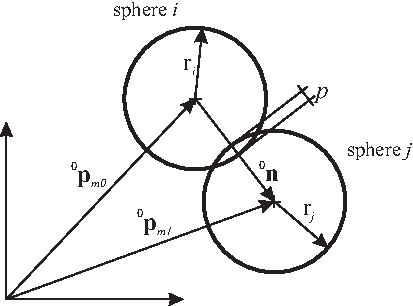
\includegraphics[width=8cm]{figures/generalContactSpheres}
  \end{center}
  \caption{Geometrical relations for contact of two spheres $i$ and $j$ with according markers $m0$ and $m1$.}
	\label{fig_GeneralContactSpheres}
\end{figure}
%++++++++++++++++++++++++
the velocities of the spheres at the contact point\footnote{In case of no friction, the angular velocities are not included in these relations},
\bea
  \LU{0}{\vv_{c,i}} &=& \LU{0}{\vv_i} + \left( \LU{0,m0}{\Am} \LU{m0}{\tomega}_{i} \right) \times 
               \left( \LU{0}{\pv_c} - \LU{0}{\pv_i} \right)
              = \LU{0}{\vv_i} + r_i \cdot \left( \LU{0,m0}{\Am} \LU{m0}{\tomega}_{i} \right) \times \LU{0}{\nv_0},\nonumber \\
  \LU{0}{\vv_{c,j}} &=& \LU{0}{\vv_j} + \left( \LU{0,m1}{\Am} \LU{m1}{\tomega}_{j} \right) \times 
               \left( \LU{0}{\pv_c} - \LU{0}{\pv_j} \right)
              = \LU{0}{\vv_j} - r_j \cdot \left( \LU{0,m1}{\Am} \LU{m1}{\tomega}_{j} \right) \times \LU{0}{\nv_0},
\eea
the velocity in contact normal direction, which can be computed from sphere's center points, 
\be
  v_n = \LU{0}{\nv_0\tp} \left( \LU{0}{\vv_j} - \LU{0}{\vv_i} \right)
      = \LU{0}{\nv_0\tp} \left( \LU{0}{\vv_{c,j}} - \LU{0}{\vv_{c,i}} \right)
  \eqComma
\ee
the velocity in tangential direction, considering the tangential velocities,
\bea
  \LU{0}{\vv_t} &=& \LU{0}{\vv_{c,j}} - \LU{0}{\vv_{c,i}} - v_n \cdot \LU{0}{\nv_0} 
  = \left( \Im - \LU{0}{\nv_0} \otimes \LU{0}{\nv_0}\right) \left(\LU{0}{\vv_{c,j}} - \LU{0}{\vv_{c,i}} \right), \nonumber \\
  &=& \left( \Im - \LU{0}{\nv_0} \otimes \LU{0}{\nv_0}\right) 
  \left( \LU{0}{\vv_j} + r_j \cdot \LU{0}{\tilde \nv_0} \LU{0,m1}{\Am} \LU{m1}{\tomega}_{j} 
        -\LU{0}{\vv_i} + r_i \cdot \LU{0}{\tilde \nv_0} \LU{0,m0}{\Am} \LU{m0}{\tomega}_{i} \right) \nonumber \\
  &=& \left( \Im - \LU{0}{\nv_0} \otimes \LU{0}{\nv_0}\right) 
  \left( \LU{0}{\vv_j} + r_j \cdot \LU{0}{\tilde \nv_0} \LU{0}{\tomega}_{j} 
        -\LU{0}{\vv_i} + r_i \cdot \LU{0}{\tilde \nv_0} \LU{0}{\tomega}_{i} \right)
  \eqComma
\eea
the effective contact stiffness coefficient based on the stiffness $k_i$ of sphere $i$ and stiffness $k_j$ of sphere $j$,
\be
  k_c = \frac{k_i \cdot k_j}{k_i + k_j} \eqComma
\ee
and the effective contact damping coefficient\footnote{Note that this simplicial damping law is used according to the idea of parallel dampers, because serial dampers would not allow to adjust damping for different particles} based on the damping $k_i$ of sphere $i$ and damping $k_j$ of sphere $j$
\be
  d_c = d_i + d_j \eqDot
\ee
The contact force (negative contact pressure) is computed from gap $g$ and normal velocity $v_n$,
\be
  f_c = k_c \cdot g + d_c \cdot v_n \eqComma
\ee
and the total vectorial contact force is computed with the help of \eq{eq_GeneralContactRegularizedFriction}, defining the friction force $\fv_f$,
\be
  \LU{0}{\fv_c} = f_c \cdot \nv_0 + \fv_f
  \eqDot
\ee
The torque due to friction for sphere $i$ and sphere $j$ results into\footnote{note that both signs are the same and that $\LU{0}{\fv_f}$ could be replaced by $\fv_c$}
\be
  \LU{0}{\ttau_{f,i}} = (-r_i \cdot \nv_0) \times \LU{0}{\fv_f}, \quad
  \LU{0}{\ttau_{f,j}} = (-r_j \cdot \nv_0) \times \LU{0}{\fv_f}
  \eqDot
\ee
%+++++++++++++++++++++++++++++++++++++++++++++++++++
\mysubsubsubsection{Generalized forces due to contact}
Based on the contact pressure and the friction forces, forces and torques are applied via the markers' Jacobians, resulting in generalized forces to whatever the marker is attached to.

The generalized forces to the marker $m0$ and $m1$ (sphere $i$ and $j$) are computed as
\bea
  \fv_{m0,LHS} = -\LU{0}{\Jm_{pos,m0}\tp} \LU{0}{\fv_c} + 
                 \LU{0}{\Jm_{rot,m0}\tp} \LU{0}{\ttau_{f,i}}, \nonumber \\
  \fv_{m1,LHS} = \LU{0}{\Jm_{pos,m1}\tp} \LU{0}{\fv_c} + 
                 \LU{0}{\Jm_{rot,m1}\tp} \LU{0}{\ttau_{f,j}} \eqDot
\eea
%+++++++++++++++++++++++++++++++++++++++++++++++++++
\mysubsubsubsection{Jacobi matrix for sphere $g_i$ and sphere $g_j$}
%
%
For implicit time integration, the (contact) Jacobian\footnote{Here, we only consider the local Jacobian related to the coordinates underlying the two markers $m0$ and $m1$; in the implementation, the parts of the Jacobian are added to the sparse system } represents the derivative of the generalized forces 
\be
  \fv_{LHS} = \vp{\fv_{m0,LHS}}{\fv_{m1,LHS}}
\ee
with respect to the generalized coordinates affected by the two markers,
\be
  \qv = \vp{\qv_{m0}}{\qv_{m1}} \eqDot
\ee
The Jacobian thus reads\footnote{{\bf NOTE} that only terms marked in {\bf\termC{green}} are currently fully implemented and terms in {\bf\termA{blue}} are approximated, while other terms are neglected}
\be
  \termA{ \Jm_{c}  = \frac{\partial \fv_{LHS}}{\partial \qv}
           = \mp{\frac{\partial \left(-\LU{0}{\Jm_{pos,m0}\tp} \LU{0}{\fv_c} + \LU{0}{\Jm_{rot,m0}\tp} \LU{0}{\ttau_{f,i}}\right)}{\partial \qv_{m0}}}
                {\frac{\partial \left(-\LU{0}{\Jm_{pos,m0}\tp} \LU{0}{\fv_c} + \LU{0}{\Jm_{rot,m0}\tp} \LU{0}{\ttau_{f,i}}\right)}{\partial \qv_{m1}}}
                {\frac{\partial \left( \LU{0}{\Jm_{pos,m1}\tp} \LU{0}{\fv_c} + \LU{0}{\Jm_{rot,m1}\tp} \LU{0}{\ttau_{f,j}}\right)}{\partial \qv_{m0}}}
                {\frac{\partial \left( \LU{0}{\Jm_{pos,m1}\tp} \LU{0}{\fv_c} + \LU{0}{\Jm_{rot,m1}\tp} \LU{0}{\ttau_{f,j}}\right)}{\partial \qv_{m1}}}}
\ee
The single terms may be expressed as
%terms with $\diamond$ are neglected in the current implementation}
\bea
  &&\termA{\frac{\partial \left(-\LU{0}{\Jm_{pos,m0}\tp} \LU{0}{\fv_c} + \LU{0}{\Jm_{rot,m0}\tp} \LU{0}{\ttau_{f,i}}\right)}{\partial \qv_{m0,1}} } = \nonumber \\
  &&-\frac{\partial \LU{0}{\Jm_{pos,m0}\tp}}{\partial \qv_{m0,1}} \LU{0}{\fv_c}
  \termC{-\LU{0}{\Jm_{pos,m0}\tp}} \termA{\frac{\partial \LU{0}{\fv_c}}{\partial \qv_{m0,1}}}
  +\frac{\partial \LU{0}{\Jm_{rot,m0}\tp}}{\partial \qv_{m0,1}} \LU{0}{\ttau_{f,i}}
  +\termC{\LU{0}{\Jm_{rot,m0}\tp}} \termA{\frac{\partial \LU{0}{\ttau_{f,i}}}{\partial \qv_{m0,1}}}
  \eqComma
\eea
and similar for $m_1$.
In order to simplify implementation (avoiding arrays with 3 indices) and improve computational efficiency, 
derivatives of Jacobians are realized as
\be
  \frac{\partial \LU{0}{\Jm_{pos,m0}\tp}}{\partial \qv_{m0}} \LU{0}{\fv_c} = 
  \frac{\partial \LU{0}{\Jm_{pos,m0}\tp} \LU{0}{\bar \fv_c}}{\partial \qv_{m0}}  
  \eqComma
\ee
in which $\LU{0}{\bar \fv_c} = \LU{0}{\fv_c}$, but assumed to be a constant and not depending on $\qv$ in the computation of derivatives.
Note that derivatives for position Jacobians, e.g., $\frac{\partial \LU{0}{\Jm_{pos,m0}\tp} \LU{0}{\bar \fv_c}}{\partial \qv_{m0}}$ or rotation
Jacobians are provided by the according markers (will be described there in the near future).

For the jacobians, we need to compute the derivatives of the following terms\footnote{terms that are implemented are marked in green; black terms are not implemented or unused}\footnote{to keep derivations short, we use $\LU{0}{\Jm_{pos}}$, which represents $-\LU{0}{\Jm_{pos,m0}}$ in case of 
$\frac{\partial }{\partial \qv_{m0}}$ and $\LU{0}{\Jm_{pos,m1}}$ in case of $\frac{\partial }{\partial \qv_{m1}}$   }:
\bi
  \item $L = \left(\LU{0}{\nv}\!\tp\LU{0}{\nv}\right)^\frac{1}{2}$:
  \be
    \termC{\diffmOI{L} =
    \diffmOI{\left(\LU{0}{\nv}\!\tp\LU{0}{\nv}\right)^\frac{1}{2} } =
    \frac{1}{L}\left(\LU{0}{\nv}\!\tp \diffmOI{\LU{0}{\nv}} \right) =
    \frac{1}{L}\left(\LU{0}{\nv}\!\tp \LU{0}{\Jm_{pos}} \right) =
    \left(\LU{0}{\nv_0}\!\tp \LU{0}{\Jm_{pos}} \right) }
  \ee
  \item $L^{-1} = \left(\LU{0}{\nv}\!\tp\LU{0}{\nv}\right)^{-\frac{1}{2}}$:
  \be
    \termC{\diffmOI{L^{-1}} =
    \diffmOI{\left(\LU{0}{\nv}\!\tp\LU{0}{\nv}\right)^{-\frac{1}{2}} } =
    -\frac{1}{ L^3}\left(\LU{0}{\nv}\!\tp \diffmOI{\LU{0}{\nv}} \right) =
    -\frac{1}{ L^2}\left(\LU{0}{\nv_0}\!\tp \LU{0}{\Jm_{pos}} \right) }
  \ee
  \item $\LU{0}{\nv} = \LU{0}{\pv}_{j} - \LU{0}{\pv}_{i}$:
  \be
    \termC{\diffmOI{\LU{0}{\nv}} = \LU{0}{\Jm_{pos}} }
  \ee
  \item $\LU{0}{\nv_0} = \frac{1}{L} \LU{0}{\nv}$:\footnote{NOTE: 
  dyadic product $\otimes$}
  %\be
    %\termC{\frac{\partial \LU{0}{\nv_0}}{\partial \qv_{m0}} =
        %\frac{1}{L^3}\left(\LU{0}{\nv} \otimes \LU{0}{\nv} \right) \LU{0}{\Jm_{pos,m0}}
        %-\frac{1}{L} \LU{0}{\Jm_{pos,m0}} 
        %=
        %\frac{1}{L}\left(\LU{0}{\nv_0} \otimes \LU{0}{\nv_0} - \Im \right)
        %\LU{0}{\Jm_{pos,m0}} 
        %}
  %\ee
  \be
    \termC{\diffmOI{\LU{0}{\nv_0}} =
        -\frac{1}{L^3}\left(\LU{0}{\nv}\otimes \LU{0}{\nv} \right) \LU{0}{\Jm_{pos}}
        +\frac{1}{L} \LU{0}{\Jm_{pos}} 
        =
        \frac{1}{L}\left(\Im - \LU{0}{\nv_0}\otimes \LU{0}{\nv_0} \right) \LU{0}{\Jm_{pos}}
        }
  \ee
  \item $g = L - r_i + r_j$:
  \be
    \termC{\diffmOI{g} = \LU{0}{\nv_0}\!\tp \LU{0}{\Jm_{pos}} } 
  \ee
  %\item $p = r_i + r_j - L$:
  %\be
    %\termC{\frac{\partial p}{\partial \qv_{m0}} = \LU{0}{\nv_0}\!\tp \LU{0}{\Jm_{pos,m0}} }
  %\ee
  %\be
    %\termC{\frac{\partial p}{\partial \qv_{m1}} = -\LU{0}{\nv_0}\!\tp \LU{0}{\Jm_{pos,m1}} } 
  %\ee
%++++++++++++++++++++++++++++++++++++++++++++++++++++++++++++++++++++++++++++++++++++++++++++
  \item $v_n = \left( \LU{0}{\vv}_j - \LU{0}{\vv}_i \right)\tp \LU{0}{\nv_0}$ ({\bf NOTE}: only valid in case that markers are attached to node or body reference point!!!):
  \be
    \termC{\diffmOI{v_n} = 
    \left( \LU{0}{\vv}_j - \LU{0}{\vv}_i \right)\tp \left(
     \frac{1}{L}\left(\Im - \LU{0}{\nv_0}\otimes \LU{0}{\nv_0} \right) \LU{0}{\Jm_{pos}}
       \right)  }
  \ee
  \be
    \termC{
    \diffmOIt{v_n} = \LU{0}{\nv_0\tp} \LU{0}{\Jm_{pos}} }
  \ee
%++++++++++++++++++++++++++++++++++++++++++++++++++++++++++++++++++++++++++++++++++++++++++++
  \item $f_c = k_c \cdot g + d_c \cdot v_n$:
  \be
    \termA{\diffmOI{f_c} } = 
    \termC{k_c \diffmOI{g} + d_c \diffmOI{v_n} } = 
    \termC{k_c \cdot \LU{0}{\nv_0}\!\tp \LU{0}{\Jm_{pos}} + d_c \cdot \left( \LU{0}{\vv}_j - \LU{0}{\vv}_i \right)\tp \left(
     \frac{1}{L}\left(\Im - \LU{0}{\nv_0}\otimes \LU{0}{\nv_0} \right) \LU{0}{\Jm_{pos}} \right)}
  \ee
  \be
    \diffmOIt{f_c} = 
     \termC{d_c \diffmOIt{v_n} =  d_c \LU{0}{\nv_0\tp} \LU{0}{\Jm_{pos}} }
  \ee
%+++++++++++++++++++++++++++++++++++++++++++++++++++++++++++++++++++++++++++++++++++++++++++
\item $\LU{0}{\vv_t} = \LU{0}{\vv_{c,j}} - \LU{0}{\vv_{c,i}} - v_n \cdot \LU{0}{\nv_0}=
\left( \Im - \LU{0}{\nv_0} \otimes \LU{0}{\nv_0}\right) \left( \LU{0}{\vv_j} -\LU{0}{\vv_i} \right) 
        + r_j \cdot \LU{0}{\tilde \nv_0} \LU{0}{\tomega}_{j} 
        + r_i \cdot \LU{0}{\tilde \nv_0} \LU{0}{\tomega}_{i}$:
%\item $\LU{0}{\vv_t} = \LU{0}{\vv_{c,j}} - \LU{0}{\vv_{c,i}} - v_n \cdot \LU{0}{\nv_0}=
%\left( \Im - \LU{0}{\nv_0} \otimes \LU{0}{\nv_0}\right) \left( \LU{0}{\vv_j} + r_j \cdot \LU{0}{\tilde \nv_0} \LU{0}{\tomega}_{j} 
        %-\LU{0}{\vv_i} + r_i \cdot \LU{0}{\tilde \nv_0} \LU{0}{\tomega}_{i} \right)$:
  %\bea
    %\frac{\partial \LU{0}{\vv_t}}{\partial \qv_{m0}} &=& 
    %-\left( \LU{0}{\vv}_j - \LU{0}{\vv}_i \right) \left( \frac{1}{L}\left(\LU{0}{\nv_0}\otimes \LU{0}{\nv_0} - \Im \right) \LU{0}{\Jm_{pos,m0}}  
         %\right) \cdot \LU{0}{\nv_0} \nonumber \\
%%
    %&&-v_n \cdot \left(\frac{1}{L}\left(\LU{0}{\nv_0}\otimes \LU{0}{\nv_0} - \Im \right) \LU{0}{\Jm_{pos,m0}} 
        %\right) + ... (\mbox{terms due to } \LU{m0,1}{\tomega}_{i,j})
  %\eea
  \bea
    \diffmOI{\LU{0}{\vv_t}} &=& 
    -\LU{0}{\nv_0} \otimes \left( \LU{0}{\vv}_j - \LU{0}{\vv}_i \right) \left(\frac{1}{L}\left(\Im - \LU{0}{\nv}\otimes \LU{0}{\nv} \right) \LU{0}{\Jm_{pos}}        \right) \nonumber\\
    && -v_n \left(\frac{1}{L}\left(\Im - \LU{0}{\nv}\otimes \LU{0}{\nv} \right) \LU{0}{\Jm_{pos}}        \right)
    -v_n \cdot \left(\frac{1}{L}\left(\Im - \LU{0}{\nv_0}\otimes \LU{0}{\nv_0} \right) \LU{0}{\Jm_{pos}} 
        \right)\nonumber \\
%
    && + r_{i,j} \cdot \left( -\frac{1}{L}\LU{0}{\tilde \tomega}_{i,j}\left(\Im - \LU{0}{\nv_0}\otimes \LU{0}{\nv_0} \right)  + \LU{0}{\tilde \nv_0} \diffmOI{\LU{0}{\tomega}_{i,j}} \right)
  \eea
  %\left( \LU{0}{\vv_j} + r_j \cdot \LU{0}{\tilde \nv_0} \LU{0}{\tomega}_{j} 
        %-\LU{0}{\vv_i} + r_i \cdot \LU{0}{\tilde \nv_0} \LU{0}{\tomega}_{i} \right)
\item velocity coordinate derivatives for $\LU{0}{\vv_t}$:
  %++++++++++++++++++++++++++++++++++++++++++++++
  %\LU{0}{\vv_t} = \left( \Im - \LU{0}{\nv_0} \otimes \LU{0}{\nv_0}\right) 
                  %\left( \LU{0}{\vv_j} + r_j \cdot \LU{0}{\tilde \nv_0} \LU{0,m1}{\Am} \LU{m1}{\tomega}_{j} 
                        %-\LU{0}{\vv_i} + r_i \cdot \LU{0}{\tilde \nv_0} \LU{0,m0}{\Am} \LU{m0}{\tomega}_{i} \right)
  \bea
    \termC{\frac{\partial \LU{0}{\vv_t}}{\partial \dot \qv_{m0}} } &=& \termC{ 
    \left( \Im - \LU{0}{\nv_0} \otimes \LU{0}{\nv_0}\right) \left(-\LU{0}{\Jm_{pos,m0}} \right)
    + r_i \cdot \LU{0}{\tilde \nv_0} \LU{0}{\Jm_{rot,m0}}
    } \eqComma
    \\
    %
    \termC{\frac{\partial \LU{0}{\vv_t}}{\partial \dot \qv_{m1}} } &=& \termC{
    \left( \Im - \LU{0}{\nv_0} \otimes \LU{0}{\nv_0}\right) \left(\LU{0}{\Jm_{pos,m1}} \right)
    + r_j \cdot \LU{0}{\tilde \nv_0} \LU{0}{\Jm_{rot,m1}} }
  \eea
\ei
%++++++++++++++++++++++++++++++++++++++++++++++++++++++++++++++++++++++++++++++++++++++++++++
The contact force reads (note that because $f_c$ is always negative, the sign of regularization term is negative),
\be
  \LU{0}{\fv_c} = f_c \cdot \LU{0}{\nv_0} + \fv_f 
                =
              \begin{cases}
                f_c \left(\LU{0}{\nv_0} - \frac{\mu_s}{v_{\mu,reg}}\LU{0}{\vv_t} \right), \quad \mathrm{if} \quad |\LU{0}{\vv_t}| < v_{\mu,reg} \\
                f_c \cdot \LU{0}{\nv_0} + \fv_f, \quad \mbox{else with $\fv_f = const.$} 
              \end{cases}
\ee
Thus we introduce a factor $\delta_f$, which is $\delta_f=1$ in the regularized small velocity state, and in the saturated (constant) friction force we use $\delta_f=0$.
Thus, the jacobian of the contact force $\LU{0}{\fv_c}$ reads (note the diadic product $\otimes$),
%
%{\Large Second Term missing, especially when almost tangential contact ...}
\bea
 \termC{ \diffmOI{\LU{0}{\fv_c}} } &=& 
   \termC{\left(\LU{0}{\nv_0} - \delta_f \frac{\mu_s}{v_{\mu,reg}}\LU{0}{\vv_t} \right) \otimes \diffmOI{f_c}+
  f_c \left(\diffmOI{\LU{0}{\nv_0}} - \delta_f \frac{\mu_s}{v_{\mu,reg}} \diffmOI{\LU{0}{\vv_t}} \right) } \nonumber \\
  %\termC{\diffmOI{\LU{0}{\fv_c}} } &= &
  &=& \termC{\left(\LU{0}{\nv_0} - \delta_f \frac{\mu_s}{v_{\mu,reg}}\LU{0}{\vv_t} \right)
         \left( k_c \diffmOI{g} + d_c \diffmOI{v_n} \right) +
        f_c \left(\diffmOI{\LU{0}{\nv_0}} - \delta_f \frac{\mu_s}{v_{\mu,reg}} \diffmOI{\LU{0}{\vv_t}} \right)
        }  \nonumber \\
  &=&
  \termC{\left(\LU{0}{\nv_0} - \delta_f \frac{\mu_s}{v_{\mu,reg}}\LU{0}{\vv_t} \right) \otimes 
         \left(k_c \cdot \LU{0}{\nv_0\tp} + d_c \cdot \left( \LU{0}{\vv}_j - \LU{0}{\vv}_i \right)\tp  
         \left( \frac{1}{L}\left(\Im - \LU{0}{\nv_0}\otimes \LU{0}{\nv_0} \right)  \right) \right) 
         \LU{0}{\Jm_{pos}}  + f_c \cdot \left( \ldots \right)  
        } 
\eea
%\be
  %\termA{\frac{\partial \LU{0}{\fv_c}}{\partial \qv_{m0}} } \approx
  %\termC{\left(\LU{0}{\nv_0} - \delta_f \frac{\mu_s}{v_{\mu,reg}}\LU{0}{\vv_t} \right)} \otimes 
  %%\termA{\frac{\partial f_c}{\partial \qv_{m0}}} %neglected
  %\termC{\left( k_c \frac{\partial g}{\partial \qv_{m0}} \right) } 
  %%- d_c \frac{\partial v_n}{\partial \qv_{m0}} %neglected
  %=
  %-k_c \termC{\left(\LU{0}{\nv_0} - \delta_f \frac{\mu_s}{v_{\mu,reg}}\LU{0}{\vv_t} \right)} \otimes 
  %\termC{\left(\LU{0}{\nv_0\tp} \LU{0}{\Jm_{pos,m0}} \right) } 
%\ee
The jacobian for the contact force $\LU{0}{\fv_c}$ w.r.t.\ velocity marker coordinates reads, note that $\LU{0}{\nv_0} \otimes \LU{0}{\nv_0} - \Im = -\left( \Im - \LU{0}{\nv_0} \otimes \LU{0}{\nv_0} \right)$,
\be
  \termC{ \frac{\partial \LU{0}{\fv_c}}{\partial \dot \qv_{m0,1}} =
  \left(\LU{0}{\nv_0} - \delta_f \frac{\mu_s}{v_{\mu,reg}}\LU{0}{\vv_t} \right) \otimes \frac{\partial \LU{0}{f_c}}{\partial \dot \qv_{m0,1}} - 
  f_c \cdot \left(\delta_f \frac{\mu_s}{v_{\mu,reg}} \frac{\partial \LU{0}{\vv_t}}{\partial \dot \qv_{m0,1}} \right) } 
\ee
\bea
  \termC{ \frac{\partial \LU{0}{\fv_c}}{\partial \dot \qv_{m0}} }
  &=&   \termC{ -d_c \left(\LU{0}{\nv_0} - \delta_f \frac{\mu_s}{v_{\mu,reg}}\LU{0}{\vv_t} \right) \otimes 
  \left( \LU{0}{\nv_0\tp} \LU{0}{\Jm_{pos,m0}}\right) - } \nonumber \\
  &&
  \termC{ f_c \cdot \delta_f \frac{\mu_s}{v_{\mu,reg}} 
  \left( -\left( \Im - \LU{0}{\nv_0} \otimes \LU{0}{\nv_0} \right) 
  \LU{0}{\Jm_{pos,m0}} + r_i \cdot \LU{0}{\tilde \nv_0} \LU{0}{\Jm_{rot,m0}} \right)
  } 
  \nonumber \\
  \termC{ \frac{\partial \LU{0}{\fv_c}}{\partial \dot \qv_{m1}} }
  &=&   \termC{ d_c \left(\LU{0}{\nv_0} - \delta_f \frac{\mu_s}{v_{\mu,reg}}\LU{0}{\vv_t} \right) \otimes 
  \left( \LU{0}{\nv_0\tp} \LU{0}{\Jm_{pos,m1}}\right) - } \nonumber \\
  &&
  \termC{ f_c \cdot \delta_f \frac{\mu_s}{v_{\mu,reg}} 
  \left( \left( \Im - \LU{0}{\nv_0} \otimes \LU{0}{\nv_0} \right) 
  \LU{0}{\Jm_{pos,m1}} + r_j \cdot \LU{0}{\tilde \nv_0} \LU{0}{\Jm_{rot,m1}} \right)
  } 
\eea

%\rowTable{relative position}{$\LU{0}{\nv}$}{$\LU{0}{\pv}_{j} - \LU{0}{\pv}_{i}$}
%\rowTable{Distance$^*$}{$L = |\LU{0}{\nv}|$}{}
%\rowTable{unit vector$^*$}{$\LU{0}{\nv_0} = \frac{1}{L} \LU{0}{\nv}$}{vector in contact normal direction}
%\rowTable{penetration$^*$}{$p = r_i + r_j - L$}{}
%v_n = \LU{0}{\nv_0} \left( \LU{0}{\vv}_j - \LU{0}{\vv}_i \right)
%\LU{0}{\vv_t} = \LU{0}{\vv}_j - \LU{0}{\vv}_i - v_n \cdot \LU{0}{\nv_0} \eqComma

%Thus, the derivative of the contact force w.r.t.\ $\qv_{m0}$ is given as
%simplifies k_c*T term, but other terms stay complicated:
%\be
  %\frac{\partial \LU{0}{\fv_c}}{\partial \qv_{m0}} = 
    %-k_c \Im_{3\times 3} + k_c(r_i + r_j) \frac{\partial \LU{0}{\nv_0}}{\partial \qv_{m0}} 
    %-2 \cdot d_c \cdot \left(\LU{0}{\nv_0} \left( \LU{0}{\vv}_j - \LU{0}{\vv}_i \right)\right) \frac{\partial \LU{0}{\nv_0}}{\partial \qv_{m0}}
    %+ \frac{\partial f_c}{\partial \qv_{m0}} \frac{\mu_s}{v_{\mu,reg}}\LU{0}{\vv_t}
    %+ f_c \frac{\partial \frac{\mu_s}{v_{\mu,reg}}\LU{0}{\vv_t}}{\partial \qv_{m0}}
%\ee
\noindent The jacobians for torques are computed for the case that friction is in the regularized small velocity state ($\delta_f=1$), while otherwise derivatives of $\LU{0}{\ttau_{f,(i,j)}}$ are zero, 
\be
  \LU{0}{\ttau_{f,i}} = (-r_i \cdot \LU{0}{\nv_0}) \times \left( -f_c \cdot\delta_f \frac{\mu_s}{v_{\mu,reg}}\LU{0}{\vv_t} \right), \quad
  \LU{0}{\ttau_{f,j}} = (-r_j \cdot \LU{0}{\nv_0}) \times \left( -f_c \cdot\delta_f \frac{\mu_s}{v_{\mu,reg}}\LU{0}{\vv_t} \right)
\ee
in case of no friction or constant friction forces, $\delta_f=0$.
The jacobians follow from (accordingly for $\ttau_{f,i}$, $\ttau_{f,j}$ and derivatives w.r.t\ $\qv_{m0,1}$):
\bea
    \frac{\partial \LU{0}{\ttau_{f,(i,j)}}}{\partial \qv_{m0,1}} 
    &=&\frac{\partial \left(-r_ {(i,j)} \cdot \LU{0}{\nv_0} \right) \times \left( -f_c \cdot \delta_f \frac{\mu_s}{v_{\mu,reg}}\LU{0}{\vv_t} \right) }{\partial \qv_{m0,1}}\nonumber \\
   &=& \left(-r_ {(i,j)} \frac{\partial \LU{0}{\nv_0}}{\partial \qv_{m0,1}}\right) \times \left( -f_c \cdot \delta_f \frac{\mu_s}{v_{\mu,reg}}\LU{0}{\vv_t} \right) +
    \left(-r_ {(i,j)} \cdot \LU{0}{\nv_0} \right) \times \left( -f_c \cdot \delta_f \frac{\mu_s}{v_{\mu,reg}} \frac{\partial \LU{0}{\vv_t}}{\partial \qv_{m0,1}}\right) + \diffmOI{f_c} (...)
    \nonumber \\
   &=& \left( -f_c \cdot \delta_f \frac{\mu_s}{v_{\mu,reg}}\LU{0}{\tilde \vv_t} \right) \left(r_ {(i,j)} \frac{\partial \LU{0}{\nv_0}}{\partial \qv_{m0,1}} \right) +
    \left(-r_ {(i,j)} \cdot \LU{0}{\tilde \nv_0} \right) \left( -f_c \cdot \delta_f \frac{\mu_s}{v_{\mu,reg}} \frac{\partial \LU{0}{\vv_t}}{\partial \qv_{m0,1}}\right) + \diffmOI{f_c} (...)
\eea
and (note that $\LU{0}{\tilde \nv_0} \LU{0}{\nv_0} = \Null$),
\bea
    \termC{ \frac{\partial \LU{0}{\ttau_{f,(i,j)}}}{\partial \dot \qv_{m0}}  }
   &=&\termC{\left(-r_ {(i,j)} \cdot \LU{0}{\tilde \nv_0} \right) \left( -f_c \cdot \delta_f \frac{\mu_s}{v_{\mu,reg}} \frac{\partial \LU{0}{\vv_t}}{\partial    \dot \qv_{m0}} - \diffmOt{f_c} \cdot \delta_f \frac{\mu_s}{v_{\mu,reg}} \LU{0}{\vv_t} \right)  } \nonumber\\
   &=&\termC{ \left(r_ {(i,j)} \cdot \LU{0}{\tilde \nv_0} \right) \left( f_c \cdot \delta_f \frac{\mu_s}{v_{\mu,reg}} 
    \left( - \LU{0}{\Jm_{pos,m0}} 
    %\left( -\left( \Im - \LU{0}{\nv_0} \otimes \LU{0}{\nv_0} \right) \LU{0}{\Jm_{pos,m0}} 
    + r_i \cdot \LU{0}{\tilde \nv_0} \LU{0}{\Jm_{rot,m0}} \right)  - d_c\delta_f \frac{\mu_s}{v_{\mu,reg}} \cdot \LU{0}{\vv_t} \otimes (\LU{0}{\nv_0} \LU{0}{\Jm_{pos,m0}} ) \right)
    }
\eea
\bea
    \termC{ \frac{\partial \LU{0}{\ttau_{f,(i,j)}}}{\partial \dot \qv_{m1}} }
   &=&\termC{\left(-r_ {(i,j)} \cdot \tilde \nv_0 \right) \left( -f_c \cdot \delta_f \frac{\mu_s}{v_{\mu,reg}} \frac{\partial \LU{0}{\vv_t}}{\partial    \dot \qv_{m1}} - \diffmIt{f_c} \cdot \delta_f \frac{\mu_s}{v_{\mu,reg}} \LU{0}{\vv_t}  \right)  } \nonumber\\
   &=&\termC{ \left(r_ {(i,j)} \cdot \tilde \nv_0 \right) \left(f_c \cdot \delta_f \frac{\mu_s}{v_{\mu,reg}} 
    \left( \LU{0}{\Jm_{pos,m1}} 
    %\left( \left( \Im - \LU{0}{\nv_0} \otimes \LU{0}{\nv_0} \right) \LU{0}{\Jm_{pos,m1}} 
    + r_j \cdot \LU{0}{\tilde \nv_0} \LU{0}{\Jm_{rot,m1}} \right) + d_c\delta_f \frac{\mu_s}{v_{\mu,reg}} \cdot \LU{0}{\vv_t} \otimes (\LU{0}{\nv_0} \LU{0}{\Jm_{pos,m1}} ) \right)
    }
\eea
%++++++++++++++++++++++++++++++++++++++++++++++++++++++++++++++++++++++++
%++++++++++++++++++++++++++++++++++++++++++++++++++++++++++++++++++++++++
%
\mysubsubsection{Contact relations for ANCF cable $g_i$ (marker $m0$) and sphere $g_j$ (marker $m1$)}
\noindent If contact is active, we have two relative axial reference coordinates $s_0$ and $s_1$, which define start and end location at the beam, for which the span in between intersects with the circle, see \fig{fig_generalContactANCF2Dcircle}.
The intersection points are either computed based on the exact 6th order polynomial equations or using a set of linear segments for interpolation.
In this model, due to the active set strategy, the reference coordinates spanning $[s_0,\, s_1]$ are kept fixed, even though that they would change during Newton iterations.
%++++++++++++++++++++++++
\begin{figure}[tbph]
  \begin{center}
  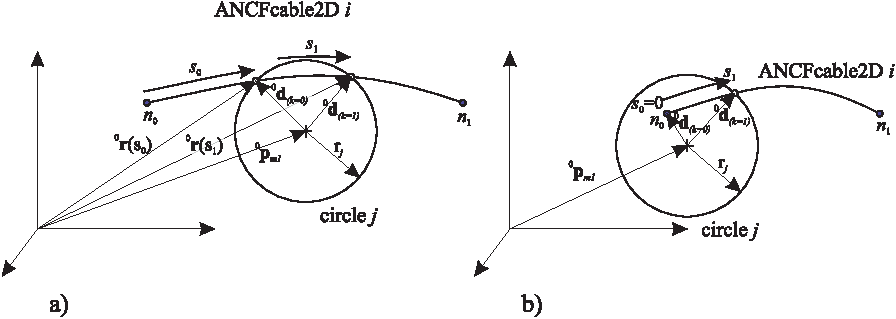
\includegraphics[width=\textwidth]{figures/generalContactANCF2Dcircle}
  \end{center}
  \caption{Geometrical relations for contact of ANCFCable2D $i$ and circle $j$ with according marker $m1$; case a) shows a cable with nodes $n_0$ and $n_1$, partially penetrating at the midspan of the cable; case b) shows the case of a cable where node $n_0$ is inside the cable.}
	\label{fig_generalContactANCF2Dcircle}
\end{figure}
%++++++++++++++++++++++++
\newcommand{\ANCFdk}{\LU{0}{\dv_k}}
\newcommand{\ANCFdkt}{\LU{0}{\dot\dv_k}}
\newcommand{\ANCFdkO}{\LU{0}{\dv_{0,k}}}
\newcommand{\ANCFdkOtp}{\LU{0}{\dv_{0,k}\tp}}
\newcommand{\diffANCFdk}{\diffANCFmI{\ANCFdk}}

Normal contact and tangential friction forces are then computed based on integrals over the coordinates $[s_0,\, s_1]$.
The integration is performed over $n_{ip}$ integration points $x_k \in [x_{i0},\, x_{i1},\, \ldots]$. In case of a 3 point Lobatto integration, we chose the integration points 
\be
  x_k \in [s_0, (s_0+s_1)/2, s_1] \eqDot
\ee
According weights are
\be
  w_k \in [1/3, 4/3, 1/3] \eqDot
\ee
The ANCF cable provides the global position of an integration point $k \in \{i0,\, i1,\, \ldots\}$ via
\be
  \LU{0}{\rv(x_{k})} = \LU{0}{\Sm(x_{k})} \qv
\ee
with ANCF shape function matrix $\Sm$ and current ANCF coordinates $\qv$.
Note that in the simplified case with linear segments, $\LU{0}{\rv(x_{k})}$ is computed from linear interpolation of the segment which is attached to the cable.
The velocity is computed in the same way,
\be
  \LU{0}{\dot \rv(x_{k})} = \LU{0}{\Sm(x_{k})} \dot\qv
\ee
again using linear interpolation of the velocities along the straight segment, if linear segments are used.

In order to perform the integration of contact forces due to penetration as well as tangential (friction) forces, we iterate over all integration points, and sum up the according generalized forces on the cable and the circle marker object.

\noindent The integration factor for integration point $k$ follows from
\be
  f_k = \frac{s_1 - s_0}{2} w_k \eqComma
\ee
assuming axial stretch of the cable element being moderately small.
The vector $\ANCFdk$ which points from the center of the circle to the cable (integration) point reads
\be
  \ANCFdk = \LU{0}{\rv(x_{k})} - \LU{0}{\pv_j} 
\ee
The velocity of the circle at the contact integration point $k$ follows as
\be
  \LU{0}{\vv_{c,k}} = \LU{0}{\vv_j} + \left( \LU{0,m0}{\Am} \LU{m0}{\tomega}_{j} \right) \times \ANCFdk
\ee
The distance $L$ between cable and circle center point, gap $g$ and the contact normal vector read
\be
  L_k = |\ANCFdk|, \quad g= L_k - (r + h_{1/2}), \quad \LU{0}{\dv_{0,k}} = \frac{1}{L_k} \ANCFdk
\ee
with the half height of the ANCF element $h_{1/2}$, which gives additional penetration. Note that this height is added on the side of the circle, which virtually represents a larger circle, behaving slightly different from a cable with thickness $h$.

\noindent The velocity in contact normal direction reads (note that we use the velocity of the circle's center point),
\be
  v_n = \LU{0}{\dv_{0,k}} \left( \LU{0}{\dot \rv(x_{k})} - \LU{0}{\vv}_j \right)
\ee
The contact force (tension! is always negative) follows in the simplistic case of a linear contact model as
\be \label{eq_GeneralContactASfc}
  f_{c,k} = k_c \cdot g  + d \cdot v_n
\ee
with contact stiffness $k_c$ and contact normal damping $d_c$.

\noindent In case of tangential friction, the tangential velocity reads
\bea
  \vv_{t,k} &=& \LU{0}{\dot \rv(x_{k})} - \LU{0}{\vv}_{c,k} - v_n \cdot \LU{0}{\dv_{0,k}}
  = \LU{0}{\dot \rv(x_{k})} - \LU{0}{\vv_j} - \left( \LU{0,m0}{\Am} \LU{m0}{\tomega}_{j} \right) \times \ANCFdk - v_n \cdot \LU{0}{\dv_{0,k}} \nonumber \\
  &=& -\left(\LU{0}{\dv_{0,k}} \otimes \LU{0}{\dv_{0,k}} -\Im \right) \left( \LU{0}{\dot \rv(x_{k})} - \LU{0}{\vv}_{c,k} \right) 
      +\LU{0}{\tilde \dv_k} \LU{0,m0}{\Am} \LU{m0}{\tomega}_{j} 
\eea
and the friction force is computed from \eq{eq_GeneralContactRegularizedFriction} using the contact pressure $-f_{c,k}$ from \eq{eq_GeneralContactASfc}, while otherwise $\LU{0}{\fv_f} = \Null$.

The force vector for the contact point for integration point $k$, including integration weight $f_k$\footnote{this is done, because all further terms are proportional to $\fv_k$.} thus reads
\be
  \LU{0}{\fv_k} = f_k \cdot \left(f_{c,k} \cdot \LU{0}{\dv_{0,k}} + \LU{0}{\fv_f} \right)
\ee
%
The total force and torque on the circle $j$ is found by summation over all integration points $k$,
\be
  \LU{0}{\fv_{circ}} = \sum_k \LU{0}{\fv_{circ,k}}  = \sum_k \LU{0}{\fv_k}, \quad
  \LU{0}{\tv_{circ}} = \sum_k \LU{0}{\tv_{circ,k}}  = \sum_k \left( r_j \cdot \LU{0}{\dv_{0,k}} \right) \times \LU{0}{\fv_k}
\ee
and the contribution to the generalized forces of the ANCF cable element (with generalized coordinates $\qv_{ANCF}$) read
\be
  \fv_{ANCF} = \sum_k \fv_{ANCF,k} = \sum_k \LU{0}{\Sm(x_{k})\tp} \cdot \LU{0}{\fv_k}
\ee
%Note that in the implementation, $f_k$ is already included in the contact force $\fv_k$.
%
The generalized \ac{LHS} forces for marker $m1$ (with generalized coordinates $\qv_{m1}$) thus read
\be
  \fv_{m1,LHS} = \LU{0}{\Jm_{pos,m1}\tp} \LU{0}{\fv_{circ}} + 
                 \LU{0}{\Jm_{rot,m1}\tp} \LU{0}{\tv_{circ}} \eqDot
\ee
The Jacobian matrix for the circle-ANCF contact on position level thus reads\footnote{terms that are implemented are marked in green; black terms are not implemented or unused},
\be
  \termA{
  \Jm_{c}  = \mp{\diffANCF{ \LU{0}{\fv_{ANCF}} }}
                {\diffmI{   \LU{0}{\fv_{ANCF}} }}
                {-\diffANCF{ \left( \LU{0}{\Jm_{pos,m1}\tp} \LU{0}{\fv_{circ}} + \LU{0}{\Jm_{rot,m1}\tp} \LU{0}{\tv_{circ}}\right)}}
                {\diffmI{ \left( \LU{0}{\Jm_{pos,m1}\tp} \LU{0}{\fv_{circ}} + \LU{0}{\Jm_{rot,m1}\tp} \LU{0}{\tv_{circ}}\right)}}
                }
\ee
and on velocity level, it follows as
\be
  \termA{
  \Jm_{c}  = \mp{\diffANCFt{ \LU{0}{\fv_{ANCF}} }}
                {\diffmIt{   \LU{0}{\fv_{ANCF}} }}
                {-\diffANCFt{ \left( \LU{0}{\Jm_{pos,m1}\tp} \LU{0}{\fv_{circ}} + \LU{0}{\Jm_{rot,m1}\tp} \LU{0}{\tv_{circ}}\right)}}
                {\diffmIt{ \left( \LU{0}{\Jm_{pos,m1}\tp} \LU{0}{\fv_{circ}} + \LU{0}{\Jm_{rot,m1}\tp} \LU{0}{\tv_{circ}}\right)}}
                }
\ee
For the calculation of the jacobian, the derivatives of the following terms are needed:
\bi
  \item $\ANCFdk = \LU{0}{\rv(x_{k})} - \LU{0}{\pv_j} $:
  \be
    \diffANCF{\ANCFdk} = \diffANCF{\LU{0}{\rv(x_{k})} - \LU{0}{\pv_j} }
    = \LU{0}{\Sm(x_{k})}
  \ee
  \be
    \diffmI{\ANCFdk} = \diffmI{\LU{0}{\rv(x_{k})} - \LU{0}{\pv_j} }
    = -\LU{0}{\Jm_{pos,m1}}
  \ee
  \item $\ANCFdkt = \LU{0}{\dot \rv(x_{k})} - \LU{0}{\dot \vv_j} $:
  \be
    \diffANCFt{\ANCFdkt} = \diffANCF{\LU{0}{\dot \rv(x_{k})} - \LU{0}{\vv_j} }
    = \LU{0}{\Sm(x_{k})}
  \ee
  \be
    \diffmIt{\ANCFdkt} = \diffmI{\LU{0}{\dot \rv(x_{k})} - \LU{0}{\vv_j} }
    = -\LU{0}{\Jm_{pos,m1}}
  \ee
  \item $L_k = |\ANCFdk| = \left(\LU{0}{\dv_k\tp} \ANCFdk \right) ^{1/2}$:
  \be
    \diffANCFmI{ |\ANCFdk| } = \frac{1}{L_k}\left(\LU{0}{\dv_k\tp} \diffANCFdk \right) =
    \ANCFdkOtp \diffANCFdk 
  \ee
  %\be
    %\diffmI{ |\ANCFdk| } = - \frac{1}{L_k}\left(\LU{0}{\dv_k\tp} \LU{0}{\Jm_{pos,m1}} \right) =
    %-\left(\ANCFdkO\!\tp \LU{0}{\Jm_{pos,m1}} \right) 
  %\ee
  \item $L_k^{-1} = \left(\LU{0}{\dv_k\tp} \ANCFdk \right) ^{-1/2}$ (note different sign as in $L$-term due to $-1/2$):
  \be
    \diffANCFmI{ L_k^{-1} } = \diffANCFmI{\left(\LU{0}{\dv_k\tp} \ANCFdk \right) ^{-1/2} } = 
    -\frac{1}{L_k}\left(\ANCFdkOtp \diffANCFdk \right)
  \ee
  %\be
    %\diffmI{ L_k^{-1} } = \diffmI{\left(\LU{0}{\dv_k\tp} \ANCFdk \right) ^{-1/2} } = 
    %\frac{1}{2\cdot L_k^3}\left(\LU{0}{\dv_k\tp} \LU{0}{\Jm_{pos,m1}} \right)
  %\ee
  %\item $L^{-1} = \left(\LU{0}{\nv}\!\tp\LU{0}{\nv}\right)^{-\frac{1}{2}}$:
  %\be
    %\termC{\frac{\partial L^{-1}}{\partial \qv_{m0}} =
    %\frac{\partial \left(\LU{0}{\nv}\!\tp\LU{0}{\nv}\right)^{-\frac{1}{2}} }{\partial \qv_{m0}} =
    %-\frac{1}{2\cdot L^3}\left(\LU{0}{\nv}\!\tp \frac{\partial \LU{0}{\nv}}{\partial \qv_{m0}} \right) =
    %\frac{1}{2\cdot L^3}\left(\LU{0}{\nv}\!\tp \LU{0}{\Jm_{pos,m0}} \right) }
  %\ee
  \item $\ANCFdkO = \frac{1}{L_k} \ANCFdk$: 
  \be
    \diffANCFmI{ \ANCFdkO } = \diffANCFmI{\frac{1}{L_k} \ANCFdk } = 
    - \frac{1}{L_k^2}\ANCFdk \otimes \left(\ANCFdkOtp \diffANCFdk \right) 
    + \frac{1}{L_k} \diffANCFdk = \frac{1}{L_k} \left(\Im - \ANCFdkO \otimes \ANCFdkO \right) \diffANCFdk
  \ee
  %\be
    %\diffmI{ \ANCFdkO } = \diffmI{\frac{1}{L_k} \ANCFdk } = 
      %\frac{1}{2\cdot L_k^3}\left(\LU{0}{\dv_k\tp} \LU{0}{\Jm_{pos,m1}} \right) \ANCFdk
    %- \frac{1}{L_k} \LU{0}{\Jm_{pos,m1}}
  %\ee
  \item $g= L_k - (r + h_{1/2})$:
  \be
    \diffANCFmI{ g } = \diffANCFmI{ L_k } =
    \ANCFdkOtp \diffANCFdk 
    %\LU{0}{\Sm(x_{k})}
  \ee
  %\be
    %\diffmI{ p } = -\frac{1}{L_k}\left(\ANCFdk\!\tp \LU{0}{\Jm_{pos,m1}} \right) =
    %-\ANCFdkO\!\tp \LU{0}{\Jm_{pos,m1}} 
  %\ee
  %+++++++++++++++++++++++++++++++++++++++++++++++++++++++++++++++++++++++++++++++++++++++++++++++++++++++++
  \item velocity at circle contact point $k$: $\LU{0}{\vv_{c,k}} = \LU{0}{\vv_j} + \left( \LU{0,m1}{\Am} \LU{m1}{\tomega}_{j} \right) \times \ANCFdk = \LU{0}{\vv_j} - \LU{0}{\tilde \dv_k} \LU{0,m1}{\Am} \LU{m1}{\tomega}_{j} $:
  \be
    \diffmIt{ \LU{0}{\vv_{c,k}} } =\LU{0}{\Jm_{pos,m1}}  - \LU{0}{\tilde \dv_k} \LU{0}{\Jm_{rot,m1}}
  \ee
  %+++++++++++++++++++++++++++++++++++++++++++++++++++++++++++++++++++++++++++++++++++++++++++++++++++++++++
  \item $v_n = \ANCFdkO \left( \LU{0}{\dot \rv(x_{k})} - \LU{0}{\vv}_{c,k} \right)$:\footnote{the approximate sign is used, because $\LU{0}{\vv}_{c,k}$ includes a normal component if ANCF cable is not fully tangential, which is not considered here.}
  \be
    \diffANCFmIt{ v_n } = \ANCFdkO \diffANCFt{\left( \LU{0}{\dot \rv(x_{k})} - \LU{0}{\vv}_{c,k} \right) } 
    \approx %because \LU{0}{\vv}_{c,k} includes normal component if ANCF cable is not fully tangential
        \ANCFdkOtp \diffANCFdk
  \ee
  %\be
    %\diffmIt{ v_n } = \ANCFdkO \diffmIt{\left( \LU{0}{\dot \rv(x_{k})} - \LU{0}{\vv}_{c,k} \right) } 
    %\approx -\ANCFdkO \LU{0}{\Jm_{pos,m1}}
  %\ee
  %+++++++++++++++++++++++++++++++++++++++++++++++++++++++++++++++++++++++++++++++++++++++++++++++++++++++++
  \item $\vv_{t,k} = \LU{0}{\dot \rv(x_{k})} - \LU{0}{\vv}_j - v_n \cdot \ANCFdkO =
  \left(\Im - \ANCFdkO \otimes \ANCFdkO \right) \left( \LU{0}{\dot \rv(x_{k})} - \LU{0}{\vv_j} \right) 
      +\LU{0}{\tilde \dv_k} \LU{0}{\tomega}_{j} $:
  \be
    \diffANCFt{\vv_{t,k} } = \left(\Im - \ANCFdkO \otimes \ANCFdkO \right) \LU{0}{\Sm(x_{k})}
  \ee
  \be
    \diffmIt{\vv_{t,k} } = -\left(\Im - \ANCFdkO \otimes \ANCFdkO \right) \LU{0}{\Jm_{pos,m1}} + \LU{0}{\tilde \dv_k} \LU{0}{\Jm_{rot,m1}}
  \ee
  %+++++++++++++++++++++++++++++++++++++++++++++++++++++++++++++++++++++++++++++++++++++++++++++++++++++++++
  \item $f_{c,k} = k_c \cdot g  + d_c \cdot v_n$:
  \be 
    \termA{ \diffANCF{ f_{c,k} } } = \termC{ k_c \cdot \diffANCF{ g } }  + d_c \cdot \diffANCF{ v_n }
    \approx \termC{ k_c \cdot \LU{0}{\dv_{k,0}\tp} \LU{0}{\Sm(x_{k})} }
  \ee
  \be 
    \termA{ \diffmI{ f_{c,k} } } = \termC{ k_c \cdot \diffmI{ p } }  + d_c \cdot \diffmI{ v_n }
    \approx \termC{ -k_c \cdot \LU{0}{\dv_{k,0}\tp} \LU{0}{\Jm_{pos,m1}} }
  \ee
  \be 
    \termC{\diffANCFt{ f_{c,k} } = d_c \cdot \diffANCFt{ v_n } = d_c \cdot \ANCFdkO \LU{0}{\Sm(x_{k})} }
  \ee  
  \be 
    \termC{\diffmIt{ f_{c,k} } = d_c \cdot \diffmIt{ v_n } = -d_c \cdot \ANCFdkO \LU{0}{\Jm_{pos,m1}} }
  \ee  
  %+++++++++++++++++++++++++++++++++++++++++++++++++++++++++++++++++++++++++++++++++++++++++++++++++++++++++
\ei
The contact force reads (note that because $f_c$ is always negative, the sign of regularization term is negative),
\be
  \LU{0}{\fv_k} = f_k \cdot \left( f_{c,k} \cdot \ANCFdkO + \fv_f \right)
                =
              \begin{cases}
                f_k \cdot f_{c,k} \left(\ANCFdkO - \frac{\mu_s}{v_{\mu,reg}}\LU{0}{\vv_t} \right), \quad \mathrm{if} \quad |\LU{0}{\vv_t}| < v_{\mu,reg} \\
                f_k \cdot \left( f_{c,k} \cdot \ANCFdkO + \fv_f \right), \quad \mbox{else with $\fv_f = const.$} 
              \end{cases}
\ee
%++++++++++++++++++++++++++
We introduce a factor $\delta_f$, which is $\delta_f=1$ in the regularized small velocity state, and in the saturated (constant) friction force we use $\delta_f=0$. Thus, the derivative of $\fv_f$, using $|f_{c,k}| = -f_{c,k}$, reads:
  \bea
    \termA{ \diffANCFmIt{\fv_f} } &=& \termA{ \delta_f \frac{\mu_s}{v_{\mu,reg}} \diffANCFmIt{ (-f_{c,k} \LU{0}{\vv_t}) } } \approx
    \termC{ -\delta_f f_{c,k} \frac{\mu_s}{v_{\mu,reg}} \diffANCFmIt{ \LU{0}{\vv_t} } } \nonumber \\
    \termC{ \diffANCFt{\fv_f} } &\approx& \termC{ -\delta_f f_{c,k} \frac{\mu_s}{v_{\mu,reg}} \left(\Im - \ANCFdkO \otimes \ANCFdkO \right) \LU{0}{\Sm(x_{k})} } \nonumber \\
    \termC{ \diffmIt{\fv_f} } &\approx& \termC{ -\delta_f f_{c,k} \frac{\mu_s}{v_{\mu,reg}} \left(-\left(\Im - \ANCFdkO \otimes \ANCFdkO \right) \LU{0}{\Jm_{pos,m1}} + \LU{0}{\tilde \dv_k} \LU{0}{\Jm_{rot,m1}} \right) }
    %+ \LU{0}{\tilde \dv_k} \LU{0}{\Jm_{rot,m1}} \right)
     %\mbox{??? minus in term 3 ???}
  \eea
%
%+++++++++++++++++++++++++++++++++++++++++++++++++++++++++++++++++++++++++++++++++++++++++++++++++++++++++
The term $\LU{0}{\fv_k}$ gives:
  \bea
    \termA{\frac{\partial \LU{0}{\fv_k}}{\partial \qv_{ANCF,m1}} } &=& 
    \termC{f_k \cdot} \left(\termA{ \left(\ANCFdkO - \frac{\mu_s}{v_{\mu,reg}}\LU{0}{\vv_t} \right) \otimes \frac{\partial f_{c,k}}{\partial \qv_{ANCF,m1}} } + 
    f_{c,k} \cdot \frac{\partial \ANCFdkO}{\partial \qv_{ANCF,m1}} +
    \diffANCFmI{\LU{0}{\fv_f}} \right)  \nonumber \\
    &\approx& \termC{f_k \cdot k_c \cdot \left( \left(\ANCFdkO - \frac{\mu_s}{v_{\mu,reg}}\LU{0}{\vv_t} \right) \otimes \ANCFdkO \diffANCFmI{\LU{0}{\dv_{k}}} \right) }
  \eea
and the velocity terms yield
  \bea
    \termA{\diffANCFt{\LU{0}{\fv_k}} } &=& 
    \termC{f_k \cdot \left(d_c \cdot \left(\ANCFdkO - \frac{\mu_s}{v_{\mu,reg}}\LU{0}{\vv_t} \right) \otimes \diffANCFt{v_n}  + 
    \diffANCFt{\LU{0}{\fv_f}} \right) } \nonumber \\
    &\approx& \termC{f_k \cdot \left( d_c \cdot \left(\ANCFdkO - \frac{\mu_s}{v_{\mu,reg}}\LU{0}{\vv_t} \right) \otimes \ANCFdkO -
    \delta_f f_{c,k} \frac{\mu_s}{v_{\mu,reg}} \left(\Im - \ANCFdkO \otimes \ANCFdkO \right) \right)\diffANCFt{\ANCFdkt}  }
  \eea
  \bea
    \termA{\diffmIt{\LU{0}{\fv_k}} } &=& 
    \termC{f_k \cdot \left(d_c \cdot \left(\ANCFdkO - \frac{\mu_s}{v_{\mu,reg}}\LU{0}{\vv_t} \right) \otimes \diffmIt{v_n}  + 
    \diffmIt{\LU{0}{\fv_f}} \right) } \nonumber \\
    &\approx& \termC{f_k \cdot \left( \left( d_c \cdot \left(\ANCFdkO - \frac{\mu_s}{v_{\mu,reg}}\LU{0}{\vv_t} \right) \otimes \ANCFdkO  -
    \delta_f f_{c,k} \frac{\mu_s}{v_{\mu,reg}} \left(\Im - \ANCFdkO \otimes \ANCFdkO\right) \right) \diffmIt{\ANCFdkt}\right.  } \nonumber\\
    && \termC{\left.  + \delta_f f_{c,k} \frac{\mu_s}{v_{\mu,reg}} \LU{0}{\tilde \dv_k} \LU{0}{\Jm_{rot,m1}} \right) }
  \eea
%++++++++++++++++++++++++++
%
The single jacobian terms w.r.t.\ $\qv_{ANCF}$ and $\qv_{m1}$ may be expressed as
%terms with $\diamond$ are neglected in the current implementation}
\bea
  &&\termA{\frac{\partial \left( \LU{0}{\Jm_{pos,m1}\tp} \LU{0}{\fv_{circ}} + \LU{0}{\Jm_{rot,m1}\tp} \LU{0}{\tv_{circ}}\right)}{\partial \qv_{ANCF,m1}}} = \nonumber \\
  &&\frac{\partial \LU{0}{\Jm_{pos,m1}\tp}}{\partial \qv_{ANCF,m1}} \LU{0}{\fv_{circ}}
  +\termC{\LU{0}{\Jm_{pos,m1}\tp}} \termA{\frac{\partial \LU{0}{\fv_{circ}}}{\partial \qv_{ANCF,m1}}}
  +\frac{\partial \LU{0}{\Jm_{rot,m1}\tp}}{\partial \qv_{m0,1}} \LU{0}{\tv_{circ}}
  +\termC{\LU{0}{\Jm_{rot,m1}\tp}} \termA{\frac{\partial \LU{0}{\tv_{circ}}}{\partial \qv_{ANCF,m1}}}
\eea
%\frac{\partial  }{\partial \qv_{ANCF,m1}}
Note that similar relations follow for the time derivatives $\frac{\partial}{\partial \dot \qv_{ANCF,m1}}\left( \right) $.

\noindent The derivatives of $\LU{0}{\fv_{ANCF}}$, $\LU{0}{\fv_{circ}}$, and 
\be
  \LU{0}{\tv_{circ}} = \sum_k r_j \cdot  \ANCFdkO \times \LU{0}{\fv_k} = 
                       \sum_k r_j \cdot  \LU{0}{\tilde \dv_{0,k}} \LU{0}{\fv_k}
\ee
follow from
%\LU{0}{\tv_{circ}} = \sum_k \LU{0}{\tv_{circ,k}}  = \sum_k \left( r_j \cdot \ANCFdkO \right) \times \cdot \LU{0}{\fv_k}
\bea
  \diffANCFmI{\LU{0}{\fv_{ANCF}} } &=& \termC{\sum_k \LU{0}{\Sm(x_{k})\tp}} \termA{\frac{\partial \LU{0}{\fv_k}}{\partial \qv_{ANCF,m1}}}, \nonumber \\
  %\termA{-\LU{0}{\Jm_{pos,m0}\tp} \frac{\partial  \LU{0}{\fv_{ANCF}} }{\partial \qv_{ANCF,m1}}}
  %\termA{\frac{\partial  \LU{0}{\fv_{ANCF}} }{\partial \qv_{ANCF,m1}}} &=& 
  %\termC{\sum_k \LU{0}{\Sm(x_{k})\tp}} \termA{\frac{\partial \LU{0}{\fv_k}}{\partial \qv_{ANCF,m1}}}, \nonumber \\
%
  \termA{\diffANCFmI{ \LU{0}{\fv_{circ}} } } &=& \termA{ \sum_k \diffANCFmI{ \LU{0}{\fv_k} } }, \nonumber \\
%
  \termA{\frac{\partial  \LU{0}{\tv_{circ}} }{\partial \qv_{ANCF,m1}}} &\approx& 
  \sum_k \left( \termC{r_j \cdot  \LU{0}{\tilde \dv_{0,k}} } \termA{\diffANCFmI{\LU{0}{\fv_k}} } - 
                r_j \cdot \LU{0}{\tilde \fv_k} \diffANCFmI{\LU{0}{\dv_{0,k}} } \right)
\eea


%+++++++++++++++++++++++++++++++++++++++++++++++++++++++++++++++++++++++++++++++++++++++++++++++++
    %\mysubsubsubsection{Connector forces}
    %%
    %The unit vector in force direction reads (raises SysError if $L=0$),
    %\be
      %\vv_{f} = \frac{1}{L} \Delta\! \LU{0}{\pv}
    %\ee
    %If \texttt{activeConnector = True}, the scalar spring force is computed as
    %\be
      %f_{SD} = k\cdot(L-L_0) + d \cdot\Delta\! \LU{0}{\vv}\tp \vv_{f} + f_{a}
    %\ee
    %If the springForceUserFunction $\mathrm{UF}$ is defined, $\fv$ instead becomes ($t$ is current time)
    %\be
      %f_{SD} = \mathrm{UF}(mbs, t, i_N, L-L_0, \Delta\! \LU{0}{\vv}\tp \vv_{f}, k, d, f_{a})
    %\ee
    %and \texttt{iN} represents the itemNumber (=objectNumber). Note that, if \texttt{activeConnector = False}, $f_{SD}$ is set to zero.
%
    %The vector of the spring-damper force applied at both markers finally reads
    %\be
      %\fv = f_{SD}\vv_{f}
    %\ee
    %The virtual work of the connector force is computed from the virtual displacement 
    %\be
      %\delta \Delta\! \LU{0}{\pv} = \delta \LU{0}{\pv}_{m1} - \delta \LU{0}{\pv}_{m0} \eqComma
    %\ee
    %and the virtual work (not the transposed version here, because the resulting generalized forces shall be a column vector,
    %\be
      %\delta W_{SD} = \fv \delta \Delta\! \LU{0}{\pv} 
      %= \left( k\cdot(L-L_0) + d \cdot\Delta\! \LU{0}{\vv}\tp \vv_{f} + f_{a} \right) \left(\delta \LU{0}{\pv}_{m1} - \delta \LU{0}{\pv}_{m0} \right)\tp \vv_{f} 
      %\eqDot
    %\ee
    %The generalized (elastic) forces thus result from
    %\be
      %\Qm_{SD} = \frac{\partial \LU{0}{\pv}}{\partial \qv_{SD}\tp} \fv 
      %\eqComma
    %\ee
    %and read for the markers $m0$ and $m1$,
    %\be
      %\Qm_{SD, m0} 
      %= -\left( k\cdot(L-L_0) + d \cdot\Delta\! \LU{0}{\vv}\tp \vv_{f} + f_{a} \right) \Jm_{pos,m0}\tp \vv_{f} , \quad
      %\Qm_{SD, m1} 
      %= \left( k\cdot(L-L_0) + d \cdot\Delta\! \LU{0}{\vv}\tp \vv_{f} + f_{a} \right) \Jm_{pos,m1}\tp \vv_{f} 
      %\eqComma    
    %\ee
    %where $\Jm_{pos,m1}$ represents the derivative of marker $m1$ w.r.t.\ its associated coordinates $\qv_{m1}$, analogously $\Jm_{pos,m0}$.
    %%
    %\mysubsubsubsection{Connector Jacobian}
    %The position-level jacobian for the connector, involving all coordinates associated with markers $m0$ and $m1$, follows from 
    %\be
      %\Jm_{SD} = \mp{\frac{\partial \Qm_{SD, m0}}{\partial \qv_{m0}} }{\frac{\partial \Qm_{SD, m0}}{\partial \qv_{m1}}}
                    %{\frac{\partial \Qm_{SD, m0}}{\partial \qv_{m1}} }{\frac{\partial \Qm_{SD, m1}}{\partial \qv_{m1}}}
    %\ee
    %and the velocity level jacobian reads
    %\be
      %\Jm_{SD,t} = \mp{\frac{\partial \Qm_{SD, m0}}{\partial \dot \qv_{m0}} }{\frac{\partial \Qm_{SD, m0}}{\partial \dot \qv_{m1}}}
                    %{\frac{\partial \Qm_{SD, m0}}{\partial \dot \qv_{m1}} }{\frac{\partial \Qm_{SD, m1}}{\partial \dot \qv_{m1}}}
    %\ee
    %The sub-Jacobians follow from
    %\be
      %\frac{\partial \Qm_{SD, m0}}{\partial \qv_{m0}} = 
       %-\frac{\partial \Jm_{pos,m0}\tp }{\partial \qv_{m0}} \vv_{f} \left( k\cdot(L-L_0) + d \cdot\Delta\! \LU{0}{\vv}\tp \vv_{f} + f_{a} \right) 
       %-\Jm_{pos,m0}\tp \frac{\partial \vv_{f} \left( k\cdot(L-L_0) + d \cdot\Delta\! \LU{0}{\vv}\tp \vv_{f} + f_{a} \right)   }{\partial \qv_{m0}} 
    %\ee
    %in which the term $\frac{\partial \Jm_{pos,m0}\tp }{\partial \dot \qv_{m0}}$ is computed from a special function provided by markers, that
    %compute the derivative of the marker jacobian times a constant vector, in this case the spring force $\fv$; this jacobian term is usually less  
    %dominant, but is included in the numerical as well as the analytical derivatives, see the general jacobian computation information.
    %
    %The other term, which is the dominant term, is computed as (dependence of velocity term on position coordinates neglected),
    %\bea
      %\frac{\partial \Qm_{SD, m0}}{\partial \qv_{m0}}
      %&=& -\Jm_{pos,m0}\tp \frac{\partial \vv_{f} \left( k\cdot(L-L_0) + d \cdot\Delta\! \LU{0}{\vv}\tp \vv_{f} + f_{a} \right)   }{\partial \qv_{m0}}
      %\nonumber \\
      %&=& -\Jm_{pos,m0}\tp \frac{\partial  \left( k\cdot \left( \Delta\! \LU{0}{\pv} - L_0 \vv_{f} \right)+ \vv_{f} \left(d \cdot \vv_{f}\tp \Delta\! \LU{0}{\vv}  + f_{a} \right) \right)   }{\partial \qv_{m0}} 
      %\nonumber \\
      %&\approx& \Jm_{pos,m0}\tp \left(k\cdot \Im - k  \frac{L_0}{L}\left(\Im - \LU{0}{\vv_{f}} \otimes \LU{0}{\vv_{f}} \right)  +\frac{1}{L}\left(\Im - \LU{0}{\vv_{f}} \otimes \LU{0}{\vv_{f}} \right) \left(d \cdot \vv_{f}\tp \Delta\! \LU{0}{\vv}  + f_{a} \right) \right)
      %\LU{0}{\Jm_{pos,m0}}
    %\eea
    %Noting that $\frac{\partial \vv_{f} }{\partial \qv_{m0}} = 
    %-\frac{1}{L}\left(\Im - \LU{0}{\vv_{f}} \otimes \LU{0}{\vv_{f}} \right) \LU{0}{\Jm_{pos,m0}}$ and 
    %$\frac{\partial \vv_{f} }{\partial \qv_{m1}} = 
    %\frac{1}{L}\left(\Im - \LU{0}{\vv_{f}} \otimes \LU{0}{\vv_{f}} \right) \LU{0}{\Jm_{pos,m1}}$.
%%
    %The Jacobian w.r.t.\ velocity coordinates follows as
    %\bea
      %\frac{\partial \Qm_{SD, m0}}{\partial \dot \qv_{m0}}
      %&=& -\Jm_{pos,m0}\tp \frac{\partial \vv_{f} \left( k\cdot(L-L_0) + d \cdot\Delta\! \LU{0}{\vv}\tp \vv_{f} + f_{a} \right)   }{\partial \dot \qv_{m0}}
      %\nonumber \\
      %&=& \Jm_{pos,m0}\tp \left(d \vv_{f} \otimes \vv_{f} \right) \LU{0}{\Jm_{pos,m0}} 
    %\eea
    %Jacobians for markers $m1$ and mixed $m0$/$m1$ terms follow analogously.
    
